\documentclass[a4paper,10pt]{report}
\usepackage{geometry}\geometry{a4paper,top=3.5cm,bottom=3.5cm,%
left=2.5cm,right=2.5cm,heightrounded,bindingoffset=0mm}
\usepackage[T1]{fontenc}
\usepackage[utf8]{inputenc}
\usepackage[italian]{babel}
\usepackage{graphicx}
\usepackage[export]{adjustbox}%Per il Frame attrono le immagini e il valign
\usepackage{subfig}
\usepackage{amsmath,amsfonts,amssymb,braket,mathrsfs}
\usepackage{float}
\usepackage{tabularx,booktabs}
\usepackage{hyperref}
\usepackage{epsfig}
\usepackage{pdfpages} %Per gli allegati
%\usepackage{minipage}
\usepackage[output-decimal-marker={,}]{siunitx}
\DeclareSIUnit \days {gg}
%ILe tre righe sotto ervono per mettere il grassetto dentro la tabelle siunitex usando \B, il rosso usando \RED, e il verde usando \GREEN
\sisetup{detect-weight,mode=text}
\usepackage{etoolbox}
\newrobustcmd\B{\DeclareFontSeriesDefault[rm]{bf}{b}\bfseries}
\newrobustcmd\RED{\DeclareFontSeriesDefault[rm]{bf}{b}\color{red}}
\newrobustcmd\GREEN{\DeclareFontSeriesDefault[rm]{bf}{b}\color{myGreen}}
%%
\usepackage{tikz}
\usepackage{pgfplots,pgfplotstable}
%\pgfplotsset{compat=1.15} %indica la versione da utilizzare per pgfplot
\usetikzlibrary{patterns} % per il tratteggio
\usepgfplotslibrary{groupplots}
\pgfplotsset{compat=newest}
%\usepackage{stanli}
\usepackage{xspace}% per lo spazio intelligente
\newcommand{\e}{\`E\xspace}  %E'
\usepackage{titlesec} % per formato custom dei titoli dei capitoli
%\usepackage{sideways}%%%
% redefinizione del formato del titolo del capitolo
      % da formato
      %   Capitolo X
      %   Titolo capitolo
      %   a formato
      %      Titolo capitolo 
	\titleformat{\chapter}
        {\normalfont\Huge\bfseries}{}{0em}{}
	\titlespacing*{\chapter}{0pt}{0in}{0.02in}
	\titlespacing*{\section}{0pt}{0.2in}{0.02in}
	\titlespacing*{\subsection}{0pt}{0.10in}{0.02in}
%serve per la didascalia di tabelle e figure:
\usepackage{caption}
\captionsetup{tableposition=top,figureposition=bottom,font=small}\captionsetup{format=hang,labelfont={bf,color=pantone186}} %didascalie a più righe allineate e il nome in grassetto
%non viene allineato a sinistra se la didascalia è corta una sola riga. PERCHé??
\usepackage{xcolor}
%serve per mettere il codice con lo sfondo grigio chiaro
\definecolor{pantone186}{RGB}{206, 17, 38} %il colore del logo UNITN
\definecolor{myGray}{gray}{0.5} %più basso più scuro è
\definecolor{myGreen}{rgb}{0.0, 0.5, 0.0}
\usepackage{listings} 
\lstset{basicstyle=\scriptsize\ttfamily,
backgroundcolor=\color{lightgray},%
boxpos=c,%
stringstyle=\itshape,		
lineskip=3pt,%
numbers=left,
numberstyle=\tiny,}
\usepackage{lscape}
\usepackage{multirow}
\usepackage{import}
%\usepackage{pythontex}
\begin{document}
%!TEX root = ../TesiTriennaleMeoliNicola.tex
\pagestyle{plain}
\thispagestyle{empty}
\begin{center}
  \begin{figure}[H]
    \centerline{
\psfig{file=IMG/logo_unitn_black_centerNEW.eps,
                        width=0.8\textwidth,trim = 0 0.9cm 0 0.5cm}}
  \end{figure}
\textcolor{pantone186}{\noindent\rule{\textwidth}{.5pt}}

  \Large\textsc{Dipartimento di Ingegneria Civile, Ambientale e Meccanica\\}
  \Large{Corso di Laurea in Ingegneria Civile
  }

  \vspace{3.7 cm} 
  %\Large\textsc{Elaborato finale\\} 
  %\vspace{1 cm} 
  \Huge\textsc{Confronto energetico tra diverse soluzioni edilizie\\}
  
  \vspace{0.2 cm}
  \Large{\it{Analisi termo igrometrica di alcuni pacchetti strutturali composti da differenti materiali. }}


  \vspace{4 cm} 
  \begin{tabular*}{\textwidth}{ l @{\extracolsep{\fill}} r }
  \Large\textsc{Docenti} & \Large\textsc{Studente}\\
  \Large{Rossano Albatici}& \Large{Nicola Meoli 186100}\\
  
  	
  	
  \end{tabular*}

  \vspace{3.1cm} 
  \textcolor{pantone186}{\noindent\rule{\textwidth}{1pt}}
    
  \Large{Anno accademico 2020/21}
  
\end{center}


\tableofcontents
%\setcounter{page}{1}
%Tabelle e figure sulla stessa pagina:
%Le aggiunge all'indice. phantomsection serve per non far casini con hyperref
\clearpage
\begingroup
   %\let\cleardoublepage\relax  % book
    \let\clearpage\relax        % report
        \listoftables
        \phantomsection
        \addcontentsline{toc}{chapter}{Elenco delle tabelle}
        %
        \listoffigures
        \phantomsection
        \addcontentsline{toc}{chapter}{Elenco delle figure}
\endgroup
%
%%%%%%%%%%
%Comandi aggiunti:
%%%%%%%%%%
\newcommand{\red}[1]{\textcolor{pantone186}{#1}}
%%%%%%%%%%%%%%%%%%%%%%%%%%%%%%%%%%
\newcommand{\TabellaNodi}[3]{%
\begin{table}[p]
        %\small
        \centering
        \caption{#1}
        \label{#2}
        \begin{tabular}{
                        c
                        c
                        S[table-format=2.2]
                        S[table-format=1.3]
                        S[table-format=1.3]
                        c
                        S[table-format=3.2]
                        S[table-format=3.2]
                        S[table-format=1.2]
                        }
            \toprule
            \multicolumn{1}{c}{\multirow{3}{*}{Condotta}} & \multicolumn{1}{c}{\multirow{3}{*}{Tratto}} & \multicolumn{1}{c}{Lunghezza}       & \multicolumn{1}{c}{Pendenza} & \multicolumn{1}{c}{Dislivello}      & \multicolumn{1}{c}{\multirow{3}{*}{Nodo}} & \multicolumn{1}{c}{Quota}           & \multicolumn{1}{c}{Quota}           & \multicolumn{1}{c}{MAX } \\
                                              &                                             & \multicolumn{1}{c}{condotta}       & \multicolumn{1}{c}{$i_G^{prog}$}             & \multicolumn{1}{c}{$\Delta h$}      &                                           & \multicolumn{1}{c}{fondo}      & \multicolumn{1}{c}{terreno}    & \multicolumn{1}{c}{depth}\\
                                              &                                             & \multicolumn{1}{c}{[\si{\metre}]} & \multicolumn{1}{c}{[--]}                 & \multicolumn{1}{c}{[\si{\metre}]} &                                           & \multicolumn{1}{c}{[\si{\metre}]} & \multicolumn{1}{c}{[\si{\metre}]} & \multicolumn{1}{c}{[\si{\metre}]}\\
        \midrule 
        \multicolumn{8}{c}{\textbf{Corso del Lavoro e della Scienza}} \\ 
        \input{#3} \\
        \bottomrule
        \end{tabular}%
        \end{table}
}
%%%%%%%%%%%%%%%%%%%%%%%%%%%%%%%%%%
\newcommand{\TabellaDiametriCondotte}[3]{%
\begin{table}[p]
        %\small
        \centering
        \caption{#1}
        \label{#2}
        \begin{tabular}{
                        c
                        c
                        S[table-format=3.2]
                        S[table-format=3.2]
                        S[table-format=1.3]
                        S[table-format=1.2]
                        S[table-format=1.1]
                        S[table-format=-1.1]}
            \toprule
            \multicolumn{1}{c}{\multirow{2}{*}{Condotta}} & \multicolumn{1}{c}{\multirow{2}{*}{A valle di}}&\multicolumn{1}{c}{Deflusso}&\multicolumn{1}{c}{Deflusso totale}&\multicolumn{1}{c}{$i_G$}&\multicolumn{1}{c}{$D_{prog}$}&\multicolumn{1}{c}{$D_{comm}$}&\multicolumn{1}{c}{Offset}\\
            & &\multicolumn{1}{c}{[\si{\litre\per\second}]}&\multicolumn{1}{c}{[\si{\litre\per\second}]}&\multicolumn{1}{c}{[--]}&\multicolumn{1}{c}{[\si{\metre}]}&\multicolumn{1}{c}{[\si{\metre}]}&\multicolumn{1}{c}{[\si{\metre}]}\\
        \midrule 
        \multicolumn{8}{c}{\textbf{Via Roberto da Sanseverino}} \\ 
        \input{#3} \\
        \bottomrule
        \end{tabular}%
        \end{table}
}
%%%%%%%%%%%%%%%%%%%%%%%%%%%%%%%%%%%%%%%%%%%%%%%%%%%%%%%%%%%%%
\newcommand{\TabellaVerificheLinkFLow}[3]{%
\begin{landscape}
\begin{table}[p] 
    \centering
    \caption{#1}
    \label{#2}
    \begin{tabular}{
        c
        S[table-format=1.1]
        S[table-format=3.2]
        c
        S[table-format=1.2]
        S[table-format=2.0]
        S[table-format=1.4]
        S[table-format=1.4]
        S[table-format=1.4]
        S[table-format=1.3]
        S[table-format=1.2]c
        @{}}
        \toprule
        \multicolumn{2}{c|}{} & \multicolumn{3}{c|}{Velocità} & \multicolumn{6}{c}{Riempimento e Autopulizia} \\
        \midrule
        %
        \multicolumn{1}{c}{\multirow{3}{*}{Condotta}} & \multicolumn{1}{c}{\multirow{2}{*}{Diametro}} & \multicolumn{1}{c}{Flusso}                     & \multicolumn{1}{c}{Ora max}        & \multicolumn{1}{c}{Massima}                    & \multicolumn{1}{c}{Riempimento}       & \multicolumn{1}{c}{$\vartheta = $ }    & \multicolumn{1}{c}{Raggio}          & \multicolumn{1}{c}{Pend.}       & \multicolumn{1}{c}{Pend.}            & \multicolumn{1}{c}{Tensione } \\
        %
                                                      &                                               & \multicolumn{1}{c}{massimo}                    & \multicolumn{1}{c}{flusso}         & \multicolumn{1}{c}{velocità}                   & \multicolumn{1}{c}{massimo $G$}       & \multicolumn{1}{c}{compl. di $\alpha$} & \multicolumn{1}{c}{idraulico $R_H$} & \multicolumn{1}{c}{fondo $i_F$} & \multicolumn{1}{c}{geometrica $i_G$} & \multicolumn{1}{c}{tangenziale $\tau$} \\
        %
                                                      & \multicolumn{1}{c}{[\si{\metre}]}           & \multicolumn{1}{c}{[\si{\litre\per\second}]} & \multicolumn{1}{c}{[\si{\hour}]} & \multicolumn{1}{c}{[\si{\metre\per\second}]} & \multicolumn{1}{c}{[\si{\percent}]} & \multicolumn{1}{c}{[\si{rad}]}       & \multicolumn{1}{c}{[\si{\metre}]} & \multicolumn{1}{c}{[--]}        & \multicolumn{1}{c}{[--]}             & \multicolumn{1}{c}{[\si{\pascal}]} \\
                                              \midrule
        \input{#3} \\
        \bottomrule
\end{tabular}%
\end{table}
\end{landscape}
}
%%%%%%%%%%%%%%%%%%%%%%%
%\chapter{Introduzione}
\section{Premessa}
La seguente relazione idraulica si pone lo scopo di progettare e dimensionare una rete di drenaggio urbano delle acque meteoriche del quartiere "Le Albere" a Sud-Ovest del centro storico di Trento (Figura \ref{fig:inquadramentoGenerale}), cercando inoltre di attenuare e ritardare il picco di piena.

%Come prima cosa si è fatto un inquadramento generale della zona tramite il software GIS OpenSource QGIS, in cui si è svolta un valutazione della zona con suddivisione in sottobacini, individuazione di lunghezze di drenaggio, superfici impermeabili e pendenze medie, come spiegato nel prossimo {\RED{paragrafo}}.

Come prima cosa si è fatto un inquadramento generale della zona tramite il software GIS OpenSource QGIS, in cui si è svolta una preliminare valutazione idrologica del terreno, come spiegato più approfonditamente nel prossimo paragrafo.

%Per ottenere il massimo risultato dalla rete si è svolto prima di tutto un inquadramento dell'area di studio andando a studiarne le caratteristiche pluviometriche. 

%Dopodiché si è eseguita l'analisi idrologica e idraulica dall'area allo stato di fatto per poi passare alla rete di smaltimento delle acque allo stato di progetto, esaminando il comportamento della rete con la presenza di sistemi di laminazione puntuali, come le vasche volano, e sistemi diffusi, come i LID.

%Nel capitolo \ref{cap:pluviometriche} si vedrà lo studio idrologico dell'area attraverso il calcolo dei parametri delle curve di possibilità pluviometriche dalle elaborazioni della stazione meteorologica delle Laste (TN), successivamente nel capitolo \ref{cap:progettoBase} si vedrà come saranno utilizzati per analizzare la situazione idrologica e idraulica della zona. A tale scopo si utilizza il software Storm Water Management Model (SWMM) prodotto dall'US-EPA.

Nel capitolo \ref{cap:pluviometriche} si otterranno i parametri delle curve di possibilità pluviometriche dalle elaborazioni della stazione meteorologica delle Laste (TN), successivamente nel capitolo \ref{cap:progettoBase} si vedrà come saranno utilizzati per analizzare la situazione idrologica e idraulica della zona. A tale scopo si utilizza il software Storm Water Management Model (SWMM) prodotto dall'US-EPA.

A questo punto verrà progettata e verificata, nel capitolo \ref{cap:ProgettoRete}, una rete di drenaggio delle acque meteoriche. Si valuterà il riempimento e la portata massima uscente per poi attenuarla attraverso l'aggiunta alla rete di sistemi di laminazione puntuali e diffusi.

Nell'ultimo paragrafo si effettuerà una stima dei costi di costruzione delle opere progettate.


%%%%%%%
\section{Valutazione dell’area di studio in QGIS}
\subsection{Inquadramento dell'area di studio}
\begin{figure}[p]
    \centering
    \includegraphics[trim=0cm 0cm 0cm 0cm,clip,frame,width=0.9\textwidth]{IMG/Inquadramento_Generale_scala1-10000.pdf} 
    \caption{Inquadramento dell'area di studio all'interno della città di Trento -- Scala 1:10\,000}
    \label{fig:inquadramentoGenerale}
\end{figure}
\begin{figure}[p]
    \centering
    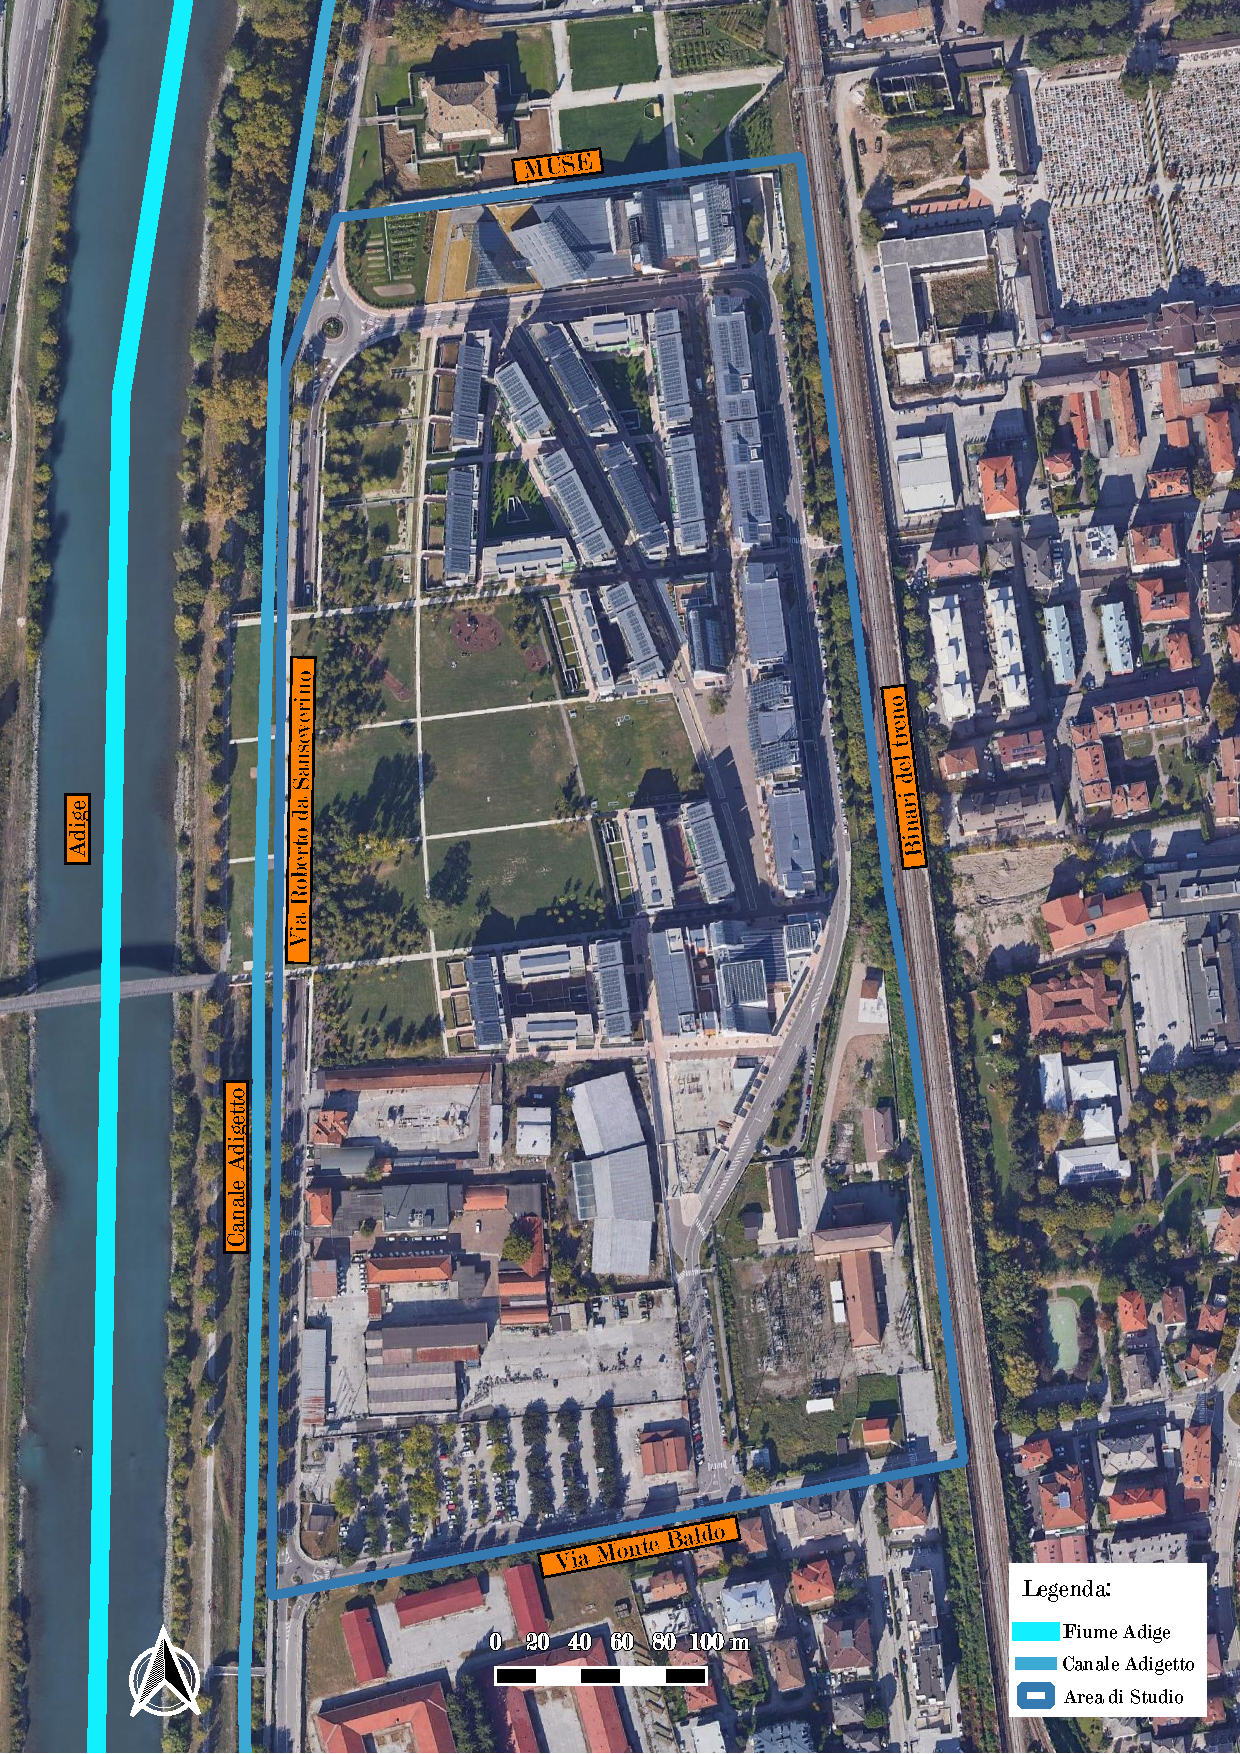
\includegraphics[trim=0cm 0cm 0cm 0cm,clip,frame,width=0.9\textwidth]{IMG/Inquadramento_scala1-2800.pdf} 
    \caption{Delimitazioni viarie e fluviali dell'area di studio -- Scala 1:2\,800}
    \label{fig:inquadramentoDettaglio}
\end{figure}

Per ottenere un ottimale inquadramento della zona si fa uso del programma QGIS sul quale dopo aver caricato le opportune mappe e aver impostato il corretto sistema di riferimento delle coordinate che, essendo l'area di studio a Trento, risulta essere WGS 84/UTM zone 32N con ID dell'autorità EPSG:32632.
Una volta immessi i dati generali su QGIS si prosegue con l'inquadramento del bacino urbano di studio.

%L'area di studio nella quale si svolge il dimensionamento della rete di drenaggio delle acque meteoriche si identifica come quartiere "Le Albere" a Sud-Ovest del centro storico di Trento (Figura \ref{fig:inquadramentoGenerale}).
La zona in esame è compresa a nord e sud tra il MUSE e Via Monte Baldo, mentre ad est e ovest rispettivamente tra i binari del treno, linea Brennero-Verona, e Via Roberto da Sanseverino (Figura \ref{fig:inquadramentoDettaglio}).
L'area si espande per un totale di circa \SI{185000}{\square\metre} e il piano campagna è compreso tra una quota di \SI{187} e \SI{194.5}{\metre \, s.l.m.}. 

Come si evince dalla figura \ref{fig:inquadramentoDettaglio} l'aria di studio è posizionata in vicinanza del fiume Adige e del canale Adigetto; fiume in cui si posizioneranno i tre recapiti finali della rete di drenaggio progettata rispettivamente a nord, al centro e a sud di via Roberto da Sanseverino.

\subsection{Sottobacini}
%Prima di procedere sul software SWMM si eseguono alcuni passaggi iniziali su QGIS. 
%%Dopo aver eseguito un primo inquadramento della zona si proseguono le operazioni iniziali per impostare la successiva analisi idrologica e idraulica dall'area.

In questa prima fase progettuale per eseguire un'analisi più precisa si è discretizzata l'area di progetto in una ventina di sottobacini. 
Questa ripartizione si svolge per ottenere un'analisi del deflusso migliore sull'area di studio (Figura \ref{fig:sottobacini}).

\begin{figure}[p]
    \centering
    \includegraphics[trim=0cm 0cm 0cm 0cm,clip,frame,width=0.9\textwidth]{IMG/sottobacini.pdf} 
    \caption{Suddivisione dell'area di studio in diversi sottobacini}
    \label{fig:sottobacini}
\end{figure}

In ciascuna suddivisione, con l'aiuto delle curve di livello, che permettono di capire la pendenza del terreno e il lato del sottobacino in cui le acque defluiscono, si realizzano le lunghezze di drenaggio. 
Queste ultime si cercano di costruirle a una distanza standard e il più perpendicolare possibile alle curve di livello.
Si determinano circa quattro lunghezze di drenaggio per sottobacino.

In seguito si ricavano e valutano i principali dati per lo svolgimento dell'analisi tra cui la pendenza media, le aree totali e le superfici impermeabili per ogni sottobacino, utili per l'analisi del drenaggio in SWMM e la successiva progettazione della rete.

%Infine si ipotizza una rete di drenaggio con l'individuazione dei nodi e delle condotte da inserire successivamente sul programma SWMM.
%%%%%%%

%\chapter{Caratteristiche pluviometriche dell’area di studio}\label{cap:pluviometriche}
\section{Curve di possibilità pluviometrica}
Dopo che si è eseguito un primo inquadramento della zona si procede con le elaborazioni dei dati dei massimi annuali degli scrosci e delle precipitazioni orarie ricavate dalla stazione pluviometrica di Laste a Trento.
Attraverso queste elaborazioni si pone l'obiettivo di determinare le curve di possibilità pluviometrica (CPP) a diversi tempi di ritorno $T_r$.
%(Tab.1 (a[mm/h alla n];n)).... svolte con il metodo di Gumbel momenti o minimi quadrati o massima verosimiglianza
Per la progettazione successiva si è scelto un tempo di ritorno di pari a \SI{25}{anni}. 

Per graficare le CPP a tempo di ritorno assegnato occorre conoscere i parametri $a$ ed $n$ della loro equazione
\begin{equation}
    \label{eq:CPP}
    h = a\,(T_r) \, t_p ^{n}
\end{equation}

Tali parametri sono ottenuti attraverso una regressione lineare tra le altezze di pioggia $h_c (T_r)$ e le durate di intensità di pioggia $t_p$. 
I parametri $a$ ed $n$ sono rispettivamente il coefficiente angolare e l'intercetta di tale regressione, visualizzata in scala logaritmica a base 10. 

Per calcolare le altezze di pioggia $h_c (T_r)$ si è fatto uso di tre metodi diversi all'interno della distribuzione di Gumbel, ovvero la probabilità di non superamento 
\begin{equation}
  P(X\leq x) = \exp{\left[-\exp{\left[-x \right]} \right]}
\end{equation}
 dove $x = \alpha ( h - u)$ mentre $h$ è il vettore con i massimi annuali relativi ad una specifica durata di precipitazione, ottenuti dalla stazione pluviometrica.

I tre diversi metodi sono:
\begin{itemize}
\item dei momenti;
\item dei minimi quadrati;
\item della massima verosimiglianza.
\end{itemize}
Avendo quindi tre diversi parametri $\alpha$ ed $u$ (avendo usato tutti e tre i metodi), per scegliere la coppia di parametri migliore si è usato il test di Pearson o del $\chi ^2$.

%si può verificare la validità delle distribuzioni ottenute tramite il test di Pearson che consiste in un test di significatività statistica.
Fatto ciò si hanno i valori dell'altezza di precipitazione per ogni tempo di ritorno per una durata fissata. 
Eseguendo il calcolo per ogni durata ed eseguendo la regressione lineare, si ottiene infine $a$ ed $n$ per poter graficare la CPP.

Nelle figure \ref{fig:ConfrontoMetodi} e \ref{fig:Pearson} viene mostrato la distribuzione di Gumbel e il relativo test di Pearson per una durata $t_p$ fissata di un'ora.
In figura \ref{fig:Regressione} è rappresentata la regressione lineare relativa ai due macro insiemi di durata (scrosci e orarie), ottenuta avendo fissato un tempo di ritorno di 25 anni. Da questo sono ottenuti i parametri $a$ ed $n$ riportati in tabella \ref{tab:parametriCPP} e da cui è stato rapresentato l'andamento delle due curve in figura \ref{fig:CPPFinale}.
\begin{table}[htbp]
    \centering
    \caption{Parametri $a$ ed $n$ per la costruzione della CPP}
    \label{tab:parametriCPP}
    \begin{tabular}{cS[table-format=2.12]S[table-format=1.12]}
            \toprule
            & $a$ & $n$ \\
            \midrule
            Scrosci & 34.890380507987 & 0.380264379496 \\
            Orarie & 32.123336325361 & 0.447173501027 \\ 
            \bottomrule
\end{tabular}
\end{table}

Da tale grafico si evince come si ottenga una maggiore altezza di precipitazione, dovuta agli scrosci, per le prime tre ore e mezza ($\hat{t}_p$) e poi le precipitazioni orarie superano gli scrosci. 
Per il seguente progetto, che riguarda un breve lasso di tempo, si prenderanno in considerazione soltanto gli scrosci. 

\begin{figure}[htbp]
    \centering
    \begin{tikzpicture}
        \begin{axis}[
            height=8cm,
            width=\textwidth,
            grid=major,
            legend pos={south east},
            xlabel=$h \, \si{[\milli\metre]}$,
            ylabel={$F, P(X\leq x)$},
            ytick = {0,0.2,0.4,0.6,0.8,1},
            %title= \emph{Vasca 2 posta a monte della condotta C21},
            /pgf/number format/.cd,
            use comma,
            1000 sep={\,}
        ]
        \addplot +[mark=*,only marks,color=green!60!black,mark options = {solid, fill=green!60!black}] table[x index=0,y index=1,header=false] {IMG/DaPython/curve__orario_1hfrequenza.txt};
        \addplot +[mark=none,style=solid,color=orange] table[x index=0,y index=1,header=false] {IMG/DaPython/curve__orario_1hmetodi.txt};
        \addplot +[mark=none,style=solid,color=magenta] table[x index=0,y index=2,header=false] {IMG/DaPython/curve__orario_1hmetodi.txt};
        \addplot +[mark=none,style=solid,color=cyan] table[x index=0,y index=3,header=false] {IMG/DaPython/curve__orario_1hmetodi.txt};
        \legend{Frequenza campionaria, Gumbel (Momenti), Gumbel (Minimi Quadrati), Gumbel (Massima Verosimiglianza)} 
        \node at (axis cs:9.7,0.9) [anchor=south west] {Durata \SI{1}{\hour}};   

        \end{axis}
    \end{tikzpicture}
    \caption{Confronto (a durata fissata) tra la frequenza campionaria e la probabilità di non superamento con i tre metodi della distribuzione di Gumbel}
    \label{fig:ConfrontoMetodi}
\end{figure}

\begin{figure}[htbp]
    \centering
    \begin{tikzpicture}
        \begin{axis}[
            height=6cm,
            width=\textwidth,
            grid=major,
            legend pos={south east},
            xlabel=$T_r \, \si{[anni]}$,
            ylabel=$h \, \si{[\milli\metre]}$,
            %ytick = {0,0.1,0.2,0.3,0.4,0.5,0.6,0.7,0.8,0.9,1},
            %title= \emph{Vasca 2 posta a monte della condotta C21},
            /pgf/number format/.cd,
            use comma,
            1000 sep={\,}
        ]
        \addplot +[mark=*,only marks,color=pantone186,mark options = {solid, fill=pantone186}] table[x index=0,y index=1,header=false] {IMG/DaPython/person__orario_1h.txt};
        \legend{{$t_p = \SI{1}{\hour}$}}    
        \end{axis}
    \end{tikzpicture}
    \caption{Andamento dell'altezza di precipitazione $h$ in funzione dei tempi di ritorno $T_r$ ottenuta dal test di Paerson per una durata $t_p$ fissata}
    \label{fig:Pearson}
\end{figure}

\begin{figure}[htbp]
    \centering
    \begin{tikzpicture}
    \begin{groupplot}[
            group style={
            %group name=my plots,
            group size=2 by 1
            %ylabels at=edge left
            },
            %restrict x to domain=-0:1.5,
            height=6cm,
            width=0.5\textwidth,
            xlabel=$t_p$ \si{[\hour]},
            ylabel=$h$  \si{[\milli\metre]},
            grid=major,
            xmode=log,
            ymode=log,
            %log ticks with fixed point,
            tick label style={
                /pgf/number format/.cd,
                use comma,
                1000 sep={\,}},
            ]
        \nextgroupplot[
            title=Scrosci]
        \addplot +[mark=none,style=solid,color=blue] table[x index=0,y index=1,header=false] {IMG/DaPython/RegressioneScrosci.txt};
        \nextgroupplot[
            title=Orarie,
            ylabel=\empty]
        \addplot +[mark=none,style=solid,color=red] table[x index=0,y index=1,header=false] {IMG/DaPython/RegressioneOrarie.txt};
    \end{groupplot}
    \end{tikzpicture}
    \caption{Regressione lineare delle altezze di pioggia con un $T_r =$ 25 anni in scala logaritmica}
    \label{fig:Regressione}
\end{figure}

\begin{figure}[htbp]
    \centering
    \begin{tikzpicture}
        \begin{axis}[
            xmin = 0, xmax = 10,
            ymin = 0, ymax = 90,
            xtick distance = 1,
            ytick distance = 10,
            height=8cm,
            width=\textwidth,
            grid=major,
            xlabel=$t_p$ \si{[\hour]},
            ylabel=$h$  \si{[\milli\metre]},
            %xtick = {0,0.5,1,1.5,2,2.5,3,3.5,4},
            %title= ,
            /pgf/number format/.cd,
            use comma,
            1000 sep={\,}
        ]
        \addplot [
            domain = 0:10,
            samples = 200,
            smooth,
            thick,
            blue,
        ]{34.890380507986976*x^0.38026437949595393};
        \addplot [
            domain = 0:10,
            samples = 200,
            smooth,
            thick,
            red,
        ]{32.123336325360924*x^0.4471735010272544};
        \legend{scrosci, orari};
        
        \draw[black,dashed] (3.438155,0) -- (3.4381,55.80218)
        node[anchor=north west] {$\hat{t}_p \simeq \SI{3.438}{\hour}$};
        \fill[] (3.4381,55.80218) circle (3pt);
        \end{axis}
    \end{tikzpicture}
    \caption{Curve di possibilità pluviometrica con i parametri $a$ ed $n$ ricavati dalla regressione logaritmica e sostituiti nell'equazione \ref{eq:CPP} con $T_r$ di 25 anni}
    \label{fig:CPPFinale}
\end{figure}
\chapter{Analisi idrologica e idraulica dell’area allo stato di fatto (valutazione del deflusso in SWMM)}\label{cap:progettoBase}
Prima di passare all'utilizzo di SWMM si è deciso quali metodologie usare all'interno dello studio.
Per la depurazione delle piogge si applica il metodo del Curve Number ($CN$) basato su Green-Ampt. 
Questo metodo utilizza le informazioni fornite dal Soil Conservation Service ($SCS-CN$), cioè il volume netto totale di un evento di pioggia e le perdite iniziali, per calibrare due parametri del modello di Green-Ampt ($GA$), ossia il tempo di "stagno (ponding)" e la conducibilità idraulica satura del suolo.
Questo metodo è vantaggioso in quanto per essere applicato richiede solamente la stima del Curve Number ($CN$) e della conducibilità idraulica ($K_s$). 
Il $CN$ si classifica in funzione del tipo e uso del suolo. 

Inoltre si valutano le portate delle condotte attraverso il modello di simulazione afflussi-deflussi e il modello di propagazione idraulica all'interno della rete nel software SWMM.

I due modelli sopra citati, per valutare i processi naturali, suddividono la zona in 3 comparti:
\begin{itemize}
\item \emph{atmosferico}, che rappresenta la precipitazione sul bacino urbano;
\item \emph{sottobacini}, creati da noi per suddividere l'area in partizioni che ricevono le acque dal comparto precedente e le indirizzano nel comparto \emph{rete di trasporto} come ruscellamento superficiale;
\item \emph{rete di trasporto}, che rappresenta l'insieme della rete: canali, tubi, vasche e LID.
\end{itemize}
A questo punto, dopo aver individualizzato le metodologie da utilizzare, si passa allo svolgimento dell'analisi idrologica e idraulica dell'area allo stato di fatto con il fine di valutare il deflusso della zona di studio.
Per elaborare queste analisi si impiega il software SWMM impostando un primo "progetto di base" per valutare i dati preliminari attraverso un modello cinematico.

Inizialmente si utilizza la figura \ref{fig:sottobacini} come sfondo su SWMM per il progetto di base andando ad inserire le coordinare che si sono ricavate precedentemente da QGIS.
Con l'aiuto dello sfondo si riportano i sottobacini inserendo in ognuno i dati in precedenza dedotti, come l'area totale, la percentuale di area impermeabile, la pendenza media e la larghezza di drenaggio calcolata come rapporto tra area [\si{\square\metre}] e lunghezza di drenaggio media [\si{\metre}] (Vedi Tabella \ref{tab:dati}).

\begin{table}[htb]
    \centering
    \caption{Dati dei sottobacini ricavati da QGIS da inserire in SWMM.}
    \label{tab:dati}
    \begin{tabular}{cS[table-format=1.4]S[table-format=3.0]S[table-format=3.2]S[table-format=1.2]}
        \toprule
        \multicolumn{1}{c}{\multirow{3}{*}{Sottobacino}} & \multicolumn{1}{c}{Area}&\multicolumn{1}{c}{Area}&\multicolumn{1}{c}{Larghezza}&\multicolumn{1}{c}{Pendenza}\\
        & \multicolumn{1}{c}{Totale}&\multicolumn{1}{c}{Impermeabile}&\multicolumn{1}{c}{Drenaggio}&\multicolumn{1}{c}{Media}\\
        & \multicolumn{1}{c}{[\si{\hectare}]} & \multicolumn{1}{c}{[\si{\percent}]}&\multicolumn{1}{c}{[\si{\metre}]}&\multicolumn{1}{c}{[\si{\percent}]}\\
        \midrule
01        & 0.3016      & 37                & 54.18               & 2.96           \\
02        & 0.6697      & 96                & 150.49              & 1.25           \\
03        & 0.3430      & 64                & 86.47               & 0.70           \\
04        & 0.5204      & 32                & 81.74               & 2.57           \\
05        & 0.3233      & 41                & 50.25               & 2.88           \\
06        & 0.9783      & 76                & 138.44              & 1.87           \\
07        & 0.8352      & 90                & 129.49              & 1.08           \\
08        & 0.7659      & 73                & 153.18              & 1.18           \\
09        & 0.3640      & 10                & 65.00               & 3.77           \\
10       & 0.6387      & 43                & 109.31              & 2.28           \\
11       & 0.5152      & 82                & 78.86               & 1.62           \\
12       & 0.3768      & 9                 & 63.86               & 3.99           \\
13       & 0.4092      & 6                 & 77.21               & 2.75           \\
14       & 0.3311      & 14                & 57.83               & 1.40           \\
15       & 0.8532      & 76                & 109.85              & 1.70           \\
16       & 0.4011      & 10                & 55.71               & 3.25           \\
17       & 0.4547      & 7                 & 60.43               & 1.29           \\
18       & 0.3676      & 83                & 59.77               & 2.18           \\
19       & 0.3808      & 27                & 61.82               & 2.84           \\
20       & 0.5283      & 77                & 93.09               & 2.03           \\
21       & 0.7326      & 82                & 93.03               & 1.89           \\
22       & 3.1032      & 100               & 197.66              & 1.59           \\
23       & 1.3079      & 70                & 108.09              & 1.21           \\
24       & 1.6037      & 85                & 187.93              & 1.16           \\
25       & 1.3684      & 79                & 139.07              & 0.93           \\ \bottomrule
\end{tabular}
\end{table}

Successivamente si costruiscono degli ietogrammi che rappresentano l'andamento dell'intensità di pioggia per una determinata durata. 
Prima si valuteranno degli ietogrammi costanti per una prima analisi grossolana e per ricavare il tempo critico.
Infine, con l'analisi dei precedenti ietogrammi, si passerà alla realizzazione del ietogramma Chicago per una rappresentazione più dettagliata e precisa dell'andamento dell'intensità di precipitazione.
% Infatti con l'inserimento di quest'ultimo ietogramma si passa dal progetto di base al progetto vero e proprio andando ad inserire su SWMM la rete di drenaggio ipotizzata su QGIS.(Fig. bo una con rete)
% In questa fase progettuale con i modelli di simulazione afflussi-deflussi e di propagazione idraulica all'interno della rete si progettano e verificano le condotte, cioè il diametro, il riempimento, l'autopulizia e la velocità dell'acqua, sistemi di laminazione puntuali, come le vasche volano, e sistemi diffusi, come i LID. 

% QUA SE VUOI AMPLIARE UN PO TE CHE STAI FACENDO QUESTA PARTI ALTRIMENTI LASCIAMO COSì O VALUTIAMO INSIEME.

% https://www.researchgate.net/publication/308697020_METODI_MISTI_DI_DEPURAZIONE_DELLA_PIOGGIA_BASATI_SUL_CURVE_NUMBER
\section{Caratteristiche dell’area allo stato di fatto}
Tenendo in considerazione la metodologia di depurazione delle acque si procede al calcolo del $CN$. 
Per fare ciò si considera una massima capacità di ritenzione idrica del suolo $S$ compresa tra \SI{85} e \SI{162}{\milli\metre} e dalla formula \ref{eq:CN} si ottiene un $CN$ tra \SI{74.92} e \SI{61.06}.
\begin{equation}
\label{eq:CN}
    CN = \frac{\SI{25400}{}}{\SI{254}{} + S}
\end{equation}
Si è deciso di applicare di applicare il valore massimo di $CN$ pari a \SI{74.92}.

Considerando che il terreno dell'area di studio sia principalmente sabbioso e con tratti ghiaiosi e limosi, attraverso la tabella 4-7 di SWMM riportata nell'appendice \ref{appendix:SWMM} a pagina \pageref{SWMM:tabella4-7} si sono scelti due parametri di conduttività idraulica $K_s$: \SI{0.43} per una classe di terreno \emph{terriccio sabbioso} e \SI{1.18} per una classe \emph{sabbia limosa}. 
Per la seguente relazione si è deciso di tener conto di un terreno con classe \emph{terriccio sabbioso}.

Infine si è proceduto al calcolo del tempo di secca $T_{\text{secco}}$, cioè il periodo di tempo che impiega il suolo completamente saturo a tornare allo stato secco.
Questo perché per la simulazione continua in SWMM richiede di specificare una stima del tempo di secca in giorni.
Utilizzando il metodo di Green-Ampt questo tempo si basa esclusivamente sulla conducibilità idraulica $K_s$ e la sua stima si calcola con la formula: 
\begin{equation}
    T_{\text{secco}} = \frac{\SI{3.125}{}}{\sqrt{K_s}}
\end{equation}
dove $K_s$ è espresso in \si{in\per\hour}.
Nel nostro caso si ha che risulta pari a \SI{4.76}{\days} per \emph{terriccio sabbioso} e \SI{2.88}{\days} per \emph{sabbia limosa}. 
Quindi in base alla classe di terreno scelta precedentemente, si è preso in considerazione il valore di \SI{4.76}{\days}.

Dopodiché per ciascuno di questi si è valutato solamente un recapito finale posto nel rivo Adigetto nella parte sud di Via Roberto da Sanseverino. 
Facendo così tutti i sottobacini creati avranno lo stesso scarico di deflusso (Figura \ref{fig:ProgettoBase}).
\begin{figure}[p]
    \centering
    \includegraphics[trim=0cm 0cm 0cm 0cm,clip,frame,width=0.9\textwidth]{IMG/ProgettoBase.pdf} 
    \caption{Posizionamento del recapito finale per verificare il deflusso dei sottobacini}
    \label{fig:ProgettoBase}
\end{figure}

Questo, come vedremo nel paragrafo successivo, ci sarà utile per la valutazione del tempo critico del bacino.

\section{Ietogramma di progetto}
Gli ietogrammi di progetto rappresentano l'andamento dell'intensità di pioggia per tutta la sua durata. Per una prima analisi grossolana si sono utilizzati ietogrammi costanti. Per elaborare i seguenti grafici si assegna un determinato tempo di ritorno, nel caso in esame pari a 25 anni, e una durata della pioggia $t_p$. 
Questi ietogrammi si eseguono per la valutazione del tempo critico del bacino urbano. Dai parametri $a$ e $n$ delle curve di possibilità pluviometriche, ricavati nel capitolo 2, si deduce l'intensità di precipitazione $i$ che viene tenuta costante per tutta la durata di pioggia dell'evento. L'intensità si ricava dalla seguente espressione:
\begin{equation}
    i = a \, t_p ^{n - 1}
\end{equation}
dove per $t_p$ si intende la durata espressa in ore. 
Si riportano in tabella \ref{tab:ietocost} i valori delle intensità di pioggia per ogni durata presa in considerazione.
\begin{table}[htbp]
    %\small
    \centering
    \caption{Intensità di precipitazione in funzione della durata}
    \label{tab:ietocost}
    \begin{tabular}{S[table-format=3.0]S[table-format=1.2]S[table-format=3.4]}
        \toprule
        \multicolumn{1}{c}{Durata} & \multicolumn{1}{c}{Durata} & \multicolumn{1}{c}{Intensità $i$}\\
        \multicolumn{1}{c}{[\si{\minute}]} & \multicolumn{1}{c}{[\si{\hour}]} & \multicolumn{1}{c}{[\si{\milli\metre\per\hour}]}\\
        \midrule
1 & 0.02 & 441.2547 \\
2 & 0.03 & 287.1642 \\
5 & 0.08 & 162.7469 \\
7 & 0.12 & 132.1150 \\
10 & 0.17 & 105.9141 \\
15 & 0.25 & 82.3804 \\
30 & 0.50 & 53.6123 \\
45 & 0.75 & 41.6999 \\
60 & 1.00 & 34.8904 \\
120 & 2.00 & 22.7063 \\
180 & 3.00 & 17.6611 \\
240 & 4.00 & 14.9275 \\
300 & 5.00 & 13.1951 \\ \bottomrule
\end{tabular}
\end{table}

Ci si è fermati ad un tempo di quattro ore perché oltre le tre ore e mezza, come visto nel capitolo \ref{cap:pluviometriche}, gli scrosci hanno meno importanza delle precipitazioni orarie.
Dopo aver calcolato i valori delle intensità, si prosegue sul programma SWMM.

Per iniziare sul progetto di base con lo scarico comune per ogni sottobacino si inseriscono i valori di intensità di precipitazione per ciascun ietogramma costante che si vuole realizzare e analizzare per valutare quale sia l'evento più gravoso e quindi il tempo critico del bacino. 
Dopodiché impostando nel pluviometro lo ietogramma costante e la rispettiva durata eseguendo il programma si ricevono i dati di picco di deflusso, di infiltrazione, di deflusso totale e di quantità di precipitazione.
Quest'ultima si può verificare facilmente dato che corrisponde all'intensità di pioggia moltiplicata per il rispettivo tempo di durata.

Ottenuti tutti i dati degli ietogrammi costanti si analizza il deflusso di ciascuno andando a constatare quale curva dia il picco maggiore e di conseguenza sapere quale sia il tempo critico del bacino (Figura \ref{fig:DeflussoBacinoIetogrammiCostanti}). 
Come si nota da questa figura il picco più gravoso e quindi l'evento meteorologico che influenza maggiormente l'area di studio si ha con una durata di pioggia di \SI{5}{\minute}.
Questo evento anche se molto breve per la nostra zona si può considerare come evento critico data la presenza di molte aree impermeabili e quindi l'area si trasforma subito in deflusso.

\begin{figure}[htb]
    \centering
    \begin{tikzpicture}
        \begin{axis}[
            restrict x to domain=-0:1.5,
            height=8cm,
            width=\textwidth,
            grid=major,
            xlabel=Tempo trascorso dall'inizio della precipitazione \si{[\hour]},
            ylabel=Deflusso  \si{[\litre\per\second]},
            xtick = {0,0.5,1,1.5,2,2.5,3,3.5,4},
            %title= ,
            /pgf/number format/.cd,
            use comma,
            1000 sep={\,}
        ]
        \addplot +[mark=none,style=solid,color=red] table[x index=0,y index=1,header=false] {IMG/Total-Inflow/total_inflow_1min.txt};
        \addplot +[mark=none,style=solid,color=green!60!black] table[x index=0,y index=1,header=false] {IMG/Total-Inflow/total_inflow_2min.txt};
        \addplot +[mark=none,style=solid,color=magenta] table[x index=0,y index=1,header=false] {IMG/Total-Inflow/total_inflow_5min.txt};
        \addplot +[mark=none,style=solid,color=cyan] table[x index=0,y index=1,header=false] {IMG/Total-Inflow/total_inflow_10min.txt};
        \addplot +[mark=none,style=solid,color=orange] table[x index=0,y index=1,header=false] {IMG/Total-Inflow/total_inflow_15min.txt};
        \addplot +[mark=none,style=solid,color=teal] table[x index=0,y index=1,header=false] {IMG/Total-Inflow/total_inflow_30min.txt};
        \addplot +[mark=none,style=solid,color=violet] table[x index=0,y index=1,header=false] {IMG/Total-Inflow/total_inflow_45min.txt};
        \legend{1 min,2 min,5 min,10 min,15 min,30 min,45 min}    
        \end{axis}
    \end{tikzpicture}
    \caption{Deflusso del bacino con l'utilizzo di ietogrammi costanti a diverse durate di pioggia. Il picco massimo è con durata di \SI{5}{\minute}}
    \label{fig:DeflussoBacinoIetogrammiCostanti}
\end{figure}

Ora per migliorare la nostra analisi dell'evento meteorologico si valuta uno ietogramma Chicago che presenta andamenti temporali non costanti e che sia di durata paragonabile o comunque maggiore all'evento critico.
Non avendo molto senso uno ietogramma Chicago pari al tempo critico di \SI{5}{\minute} dato che con un tempo così ridotto non si otterrebbero dati molto significativi, si impone una durata   $t_{\text{tot}} = \SI{2}{\hour}$, per sollecitare l'area gradualmente, e una posizione di picco $r$, che generalmente nei bacini urbani è compresa tra \SI{0.3} e \SI{0.5}, a \SI{0.5} per essere più cautelativi. 
\begin{equation}
    t_\text{picco} = {r\,t_\text{tot}}
\end{equation}
Facendo così la posizione del picco del deflusso risulterà a \SI{1}{\hour} come visibile nello ietrogramma Chicago riportato in figura \ref{fig:Chicago}.

\begin{figure}[htb]
    \centering
    \begin{tikzpicture}
        \begin{axis}[
            restrict x to domain=-0:120,
            height=6cm,
            width=\textwidth,
            grid=major,
            xlabel=Tempo trascorso dall'inizio della precipitazione \si{[\minute]},
            ylabel=Intensità di pioggia  \si{[\milli\metre\per\hour]},
            %xtick = {0,0.5,1,1.5,2,2.5,3,3.5,4},
            %title= ,
            /pgf/number format/.cd,
            use comma,
            1000 sep={\,}
        ]
        \addplot +[ybar,
            mark=none,
            enlargelimits=0.15
            style=solid,
            fill,
            color=pantone186,
            xtick=data,
            %nodes near coords,
            %nodes near coords align={vertical}
            ] 
        table[x index=0,y index=1,header=false] {IMG/Total-Inflow/chicago.txt};
        \end{axis}
    \end{tikzpicture}
    \caption{Ietogramma Chicago con $T_R = 25$ anni}
    \label{fig:Chicago}
\end{figure}   

Discretizzando lo ietogramma Chicago ad intervalli di \SI{5}{\minute}, dalla figura, si osserva una prima fase di accumulo d'acqua, dove le depressioni superficiali iniziano a colmarsi, quindi prima del picco si ha che la zona è già stata in parte sollecitata.
La costruzione del ietogramma Chicago avviene attraverso le formule dell'altezza di pioggia $h(t)$ pre e post picco e l'intensità di pioggia media $i_m$, che risulterà costante a tratti di \SI{5}{\minute}.
\begin{equation}
\label{eq:altezza}
    h(t) = 
    \begin{cases}
        r \, a \left[ \left( \frac{t_p}{r}\right)^n - \left( \frac{t_p - t}{r}\right)^n  \right] & \text{se $t < t_p$}\\
        a \left[ r \left( \frac{t_p}{r}\right)^n + (1-r)\left( \frac{t_p - t}{1 - r}\right)^n  \right] & \text{se $t > t_p$}\\
    \end{cases}
\end{equation}
\begin{equation}
\label{eq:imedia}
    i_m = \frac{h(t_\text{fin}) - h(t_\text{in})}{\Delta t}
\end{equation}
Ricavati tutti i dati necessari dello ietogramma Chicago li si riportano nel programma SWMM per ottenere i risultati dell'area di studio.

\section{Risultati dell'analisi}
%Riportare i risultati della simulazione idraulica mostrando l’idrogramma di piena in uscita dall’area di studio. Riportare in maniera esplicita il valore di colmo dell’onda di piena, il coefficiente di deflusso e il coefficiente udometrico nello stato di fatto (portata al colmo diviso area (l/s/ha). Riportare anche una breve valutazione del deflusso dei vari sottobacini.
Per la determinazione dell'ideogramma di piena in uscita dell'area di studio, riportando anche il valore di colmo dell'onda di piena, si è applicato il metodo dell'invaso lineare. 
Questo modello analizza il comportamento del bacino soggetto ad afflussi e deflussi dipendenti dal tempo e dalle caratteristiche idrauliche dello sbocco.
Lo scopo del metodo è ricavare la legge dell'andamento delle portate uscenti nel corso del tempo.
Per fare questo si prende in considerazione l'equazione di conservazione della massa:
\begin{equation}
    Q_\text{in} - Q_\text{out} = \frac{dV}{dt}
\end{equation}
dove $V$ è il volume invasato, $Q_\text{in}$ e $Q_\text{out}$ sono le portate in ingresso e in uscita e la prima di queste due si calcola come prodotto tra il coefficiente d’afflusso, l’intensità di pioggia e la superficie del bacino.
Normalizzando l'equazione precedente si ottiene:
\begin{equation}
    \delta(t) - u(t) = \frac{d\nu}{dt}
\end{equation}
dove $\delta(t)$ è il delta di Dirac, cioè la risposta del sistema all'impulso unitario, $\nu$ è il volume normalizzato, che equivale al prodotto tra la portata uscente $u(t)$ e il tempo medio di resistenza $k$ dell'acqua all'interno del sistema.
Per un tempo maggiore di zero come soluzione si ha che la funzione di trasferimento è:
\begin{equation}
    u(t) = \frac{1}{k} \, \exp{\left(-\frac{t}{k}\right)}
\end{equation}
%
\begin{table}[htbp]
    %\small
    \centering
    \caption{Dati di afflusso del progetto di base con ietogramma Chicago}
    \label{tab:afflussobase}
    \begin{tabular}{cS[table-format=2.2]S[table-format=3.2]S[table-format=1.4]S[table-format=1.2]S[table-format=3.2]}
        \toprule
        \multirow{3}{*}{Sottobacino} & \multicolumn{1}{c}{Quantità} & \multicolumn{1}{c}{Picco} & \multicolumn{1}{c}{Area} & \multicolumn{1}{c}{Coefficiente} & \multicolumn{1}{c}{Coefficiente} \\
        & \multicolumn{1}{c}{Precipitazione} & \multicolumn{1}{c}{Deflusso} & \multicolumn{1}{c}{Totale} & \multicolumn{1}{c}{Deflusso} & \multicolumn{1}{c}{Udumetrico} \\
        & \multicolumn{1}{c}{[\si{\milli\metre}]} & \multicolumn{1}{c}{[\si{\litre\per\second}]} & \multicolumn{1}{c}{[\si{\hectare}]} & \multicolumn{1}{c}{[--]} & \multicolumn{1}{c}{[\si{\litre\per\second\per\hectare}]} \\
        \midrule
01 & 45.41 & 24.43 & 0.3016 & 0.46 & 81.00 \\
02 & 45.41 & 134.42 & 0.6697 & 0.94 & 200.72 \\
03 & 45.41 & 46.50 & 0.3430 & 0.68 & 135.57 \\
04 & 45.41 & 36.59 & 0.5204 & 0.42 & 70.31 \\
05 & 45.41 & 28.97 & 0.3233 & 0.50 & 89.61 \\
06 & 45.41 & 156.16 & 0.9783 & 0.78 & 159.62 \\
07 & 45.41 & 155.90 & 0.8352 & 0.89 & 186.66 \\
08 & 45.41 & 117.87 & 0.7659 & 0.75 & 153.90 \\
09 & 45.41 & 9.13 & 0.3640 & 0.24 & 25.08 \\
10 & 45.41 & 59.42 & 0.6387 & 0.51 & 93.03 \\
11 & 45.41 & 88.38 & 0.5152 & 0.82 & 171.55 \\
12 & 45.41 & 8.86 & 0.3768 & 0.23 & 23.51 \\
13 & 45.41 & 8.74 & 0.4092 & 0.21 & 21.36 \\
14 & 45.41 & 10.94 & 0.3311 & 0.27 & 33.04 \\
15 & 45.41 & 135.41 & 0.8532 & 0.78 & 158.71 \\
16 & 45.41 & 9.78 & 0.4011 & 0.23 & 24.38 \\
17 & 45.41 & 8.12 & 0.4547 & 0.20 & 17.86 \\
18 & 45.41 & 64.46 & 0.3676 & 0.84 & 175.35 \\
19 & 45.41 & 23.14 & 0.3808 & 0.38 & 60.77 \\
20 & 45.41 & 85.69 & 0.5283 & 0.78 & 162.20 \\
21 & 45.41 & 124.96 & 0.7326 & 0.82 & 170.57 \\
22 & 45.41 & 597.69 & 3.1032 & 0.96 & 192.60 \\
23 & 45.41 & 186.08 & 1.3079 & 0.72 & 142.27 \\
24 & 45.41 & 279.28 & 1.6037 & 0.85 & 174.15 \\
25 & 45.41 & 219.56 & 1.3684 & 0.80 & 160.45 \\ \bottomrule
\end{tabular}
\end{table}

\begin{figure}[htbp]
    \centering
    \begin{tikzpicture}
        \begin{axis}[
            restrict x to domain=-0:4,
            height=8cm,
            width=\textwidth,
            grid=major,
            xlabel=Tempo trascorso dall'inizio della precipitazione \si{[\hour]},
            ylabel=Deflusso  \si{[\litre\per\second]},
            xtick = {0,0.5,1,1.5,2,2.5,3,3.5,4},
            %title= ,
            /pgf/number format/.cd,
            use comma,
            1000 sep={\,}
        ]
        \addplot +[mark=none,style=solid,color=red] table[x index=0,y index=1,header=false] {IMG/Total-Inflow/total_inflow_5min_Chicago_25anni-barato.txt};
        \node at (axis cs:1.2,2550) [anchor=south west] {\SI{2610.67}{\litre\per\second}};
        \end{axis}
    \end{tikzpicture}
    \caption{Ideogramma di piena in uscita con indicazione del picco in riferimento allo scarico di figura \ref{fig:ProgettoBase}}
    \label{fig:IdeogrammaPiena}
\end{figure}   

\begin{figure}[htbp]
    \centering
    \begin{tikzpicture}
        \begin{axis}[
            restrict x to domain=-0:4,
            height=8cm,
            width=\textwidth,
            grid=major,
            xlabel=Tempo trascorso dall'inizio della precipitazione \si{[\hour]},
            ylabel=Deflusso  \si{[\litre\per\second]},
            xtick = {0,0.5,1,1.5,2,2.5,3,3.5,4,4.5,5,5.5,6},
            /pgf/number format/.cd,
            use comma,
            1000 sep={\,}
        ]
        \addplot +[mark=none,style=solid,color=red] table[x index=0,y index=1,header=false] {IMG/Total-Inflow/deflussobarato_sottobacini_indicativi_25_20_18_6_4.txt};
        \addplot +[mark=none,style=solid,color=green!60!black] table[x index=0,y index=2,header=false] {IMG/Total-Inflow/deflussobarato_sottobacini_indicativi_25_20_18_6_4.txt};
        \addplot +[mark=none,style=solid,color=magenta] table[x index=0,y index=3,header=false] {IMG/Total-Inflow/deflussobarato_sottobacini_indicativi_25_20_18_6_4.txt};
        \addplot +[mark=none,style=solid,color=cyan] table[x index=0,y index=4,header=false] {IMG/Total-Inflow/deflussobarato_sottobacini_indicativi_25_20_18_6_4.txt};
        \addplot +[mark=none,style=solid,color=orange] table[x index=0,y index=5,header=false] {IMG/Total-Inflow/deflussobarato_sottobacini_indicativi_25_20_18_6_4.txt};
        \legend{S25,S20,S18,S6,S4}    
        \end{axis}
    \end{tikzpicture}
    \caption{Deflusso dei sottobacini più significativi con lo ietogramma chicago come input}
    \label{fig:DeflussoSottobaciniChicago}
\end{figure}   
Impostato tale modello in SWMM con tempo di ritorno pari a 25 anni si ottengono i risultati significativi dell'analisi del progetto fino ad ora.
%Eseguendo la simulazione idraulica attraverso il metodo dell'invaso lineare, riportato sopra, con tempo di ritorno pari a 25 anni si sono riportati i dati significativi del progetto.
Il primo si ha nell'ideogramma di piena in uscita con indicazione del picco di deflusso di figura \ref{fig:IdeogrammaPiena}.
Dopodiché in tabella \ref{tab:afflussobase} si hanno per ogni sottobacino il coefficiente di deflusso e il coefficiente udometrico.
Infine è riportato graficamente in figura \ref{fig:DeflussoSottobaciniChicago} l'andamento del deflusso per i sottobacini più significativi dalla quale si evince come vari il deflusso in base alla loro grandezza, alle aree verdi ed alle aree impermeabili presenti all'interno di ciascuno di essi. 
Quest'ultima se in grandi quantità genera un picco maggiore del deflusso, mentre le aree verdi e una grandezza ridotta del sottobacino danno vita a un picco di deflusso minore.
%\input{CHAPTERS/chap4_ProgettoRete.tex}
%\appendix
\chapter{Allegati}
\phantomsection
\label{appendix:SWMM}
\section{Tabelle e immagini da SWMM}
\begin{figure}[H]
    \centering
    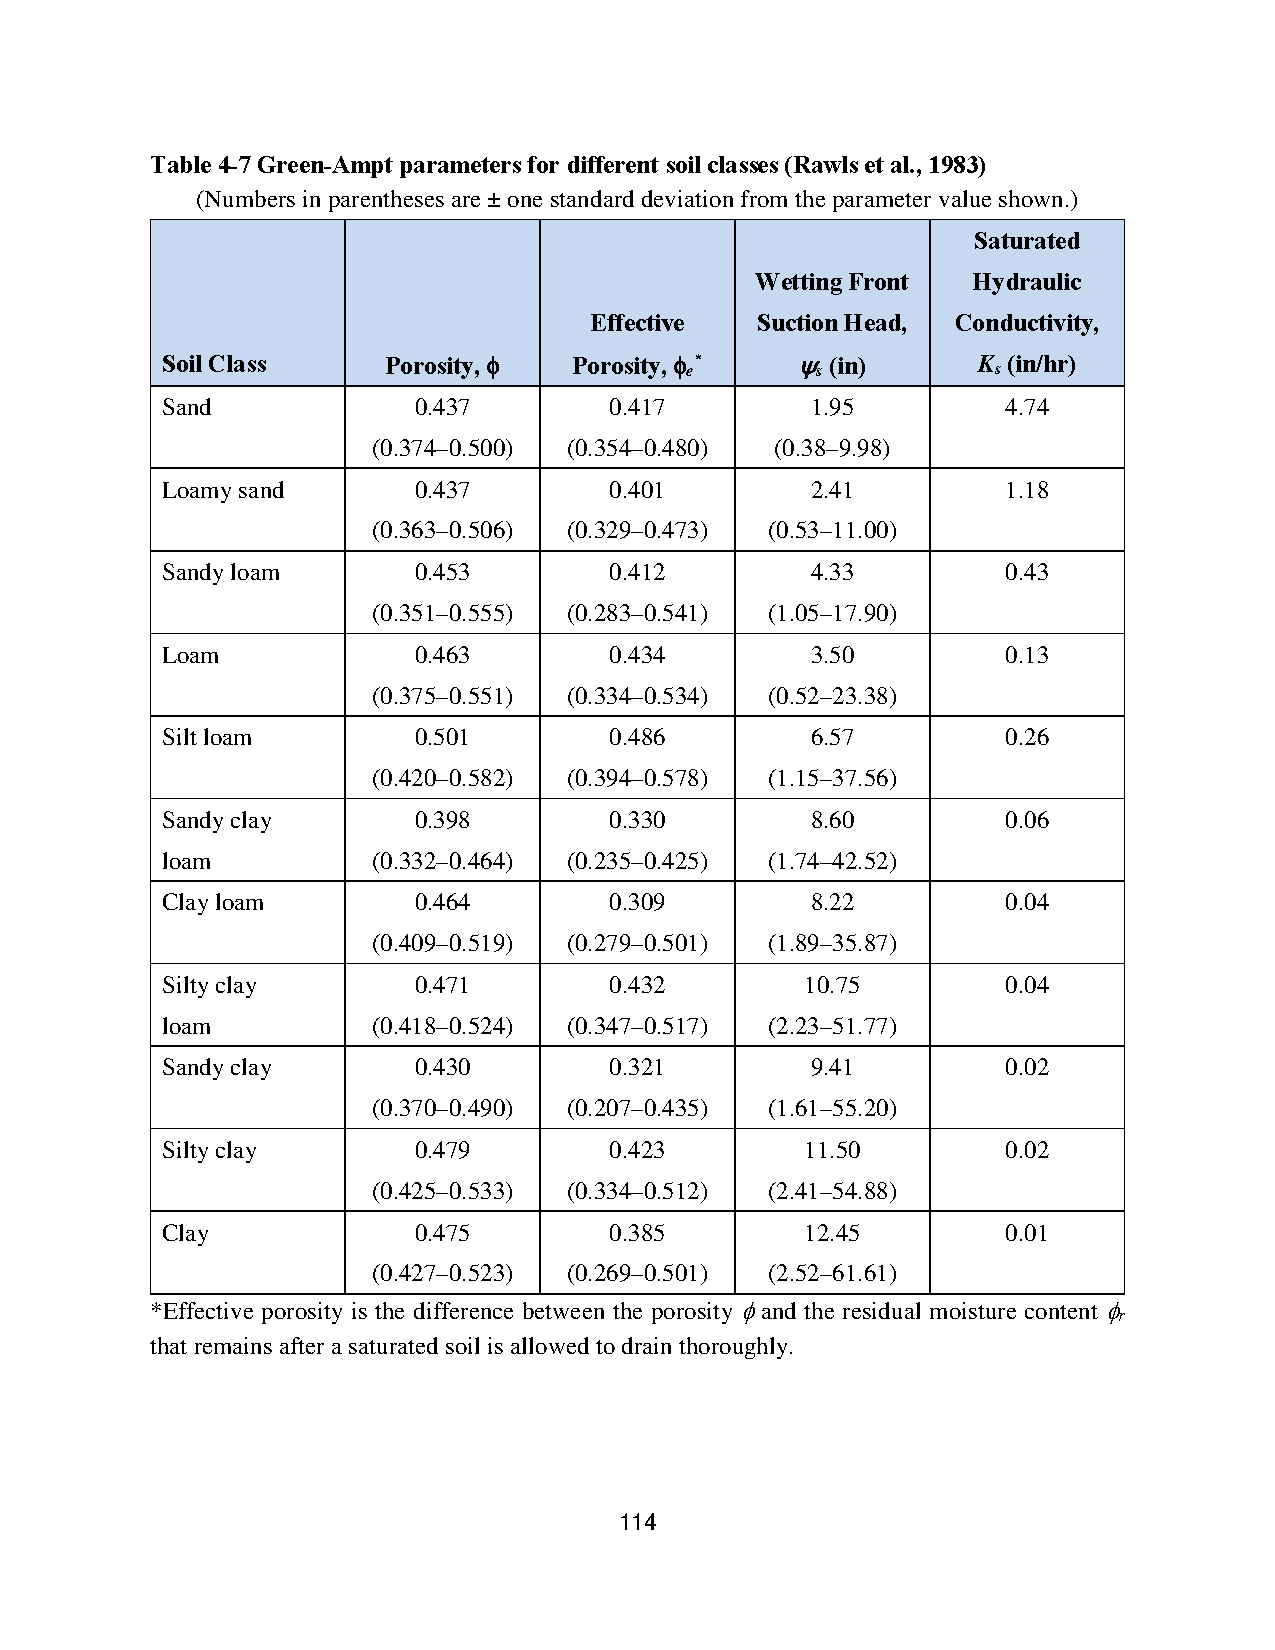
\includegraphics[trim=2.5cm 4.5cm 2.5cm 3.6cm,clip,width=\textwidth]{IMG/table4-7_Ks.pdf} 
    \caption[Tabella 4.7 di SWMM]{Tabella 4.7 di SWMM Green-Ampt parameters for different soil classes (Rawls et al., 1983) (Numbers in parentheses are ± one standard deviation from the parameter value shown.)}
    \label{SWMM:tabella4-7}
\end{figure}

%\chapter{Rete di smaltimento delle acque meteoriche allo stato di progetto (con presenza della rete di drenaggio) - tutti i mancanti}
%\label{appendix:FasiIntermedie}
%\section{Progetto sbagliato}
%\section{Progetto con solo i LID}
%\TabellaDiametriCondotte{Diametri progetti conduct-mod LID. In verde sono indicati i valori che hanno subito una modifica rispetto al progetto senza LID}{tab:Diametri_conduct-mod-LID}{IMG/Diametri-conduct-mod-LID.tex}
%\TabellaVerificheLinkFLow{Progetto con aggiunta dei soli LID -- Verifiche di massima velocità, riempimento condotta e del criterio di autopulizia}{tab:LinkFlow_Verifiche-MOD-LID}{IMG/LinkFlow-Verifiche-MOD-LID.tex}
%\section{Progetto con vasche e lid rifatto dopo i lid}
%\section{Progetto con vasche e lid sistemato}
%
\section{Codici di input SWMM per i LID e relative immagini}
\label{appendix:codiceLID}
\begin{lstlisting}
    [LID_CONTROLS]
    ;;Name               Type/Layer Parameters
    ;;--------------     ---------- ----------
    ParcheggiPermeabile1 PP
    ParcheggiPermeabile1 SURFACE    0.0        0     0.1   0.5  5
    ParcheggiPermeabile1 PAVEMENT   150        0.15  0.4   360  0     0    0
    ParcheggiPermeabile1 STORAGE    300        0.3   0.5   0
    ParcheggiPermeabile1 DRAIN      0          0.5   6     6    0     0
    TettiVerdi           GR
    TettiVerdi           SURFACE    0.0        0.0   0.1   1.0  5
    TettiVerdi           SOIL       100        0.5   0.4   0.1  2000  40   70
    TettiVerdi           DRAINMAT   50         0.3   0.01
    RetentionCellsPiante BC
    RetentionCellsPiante SURFACE    100        0.1   0.1   0.5  5
    RetentionCellsPiante SOIL       300        0.5   0.2   0.1  4     35   3.5
    RetentionCellsPiante STORAGE    200        0.75  0.5   0
    RetentionCellsPiante DRAIN      0          0.5   6     6    0     0
\end{lstlisting}
%
\begin{landscape}
\begin{lstlisting}[basicstyle=\scriptsize\ttfamily,numberstyle=\tiny]
    [LID_USAGE]
    ;;Subcatchment   LID                  Process Number     Area    Width  InitSat  FromImp  ToPerv  RptFile  DrainTo  FromPerv
    ;;-------------- ----------------     ------- ---------  ------  -----  -------  -------  ------  -------- --------
    S_2              TettiVerdi           1       1148.864   24.010  0      0        0        *       *        0
    S_2              RetentionCellsPiante 1       1233.037   32      0      0        0        *       *        0
    S_3              TettiVerdi           1       160.533    6.981   0      0        0        *       *        0
    S_4              RetentionCellsPiante 1       337.869    69.486  0      0        0        *       *        0
    S_5              RetentionCellsPiante 1       147.403    36.546  0      0        0        *       *        0
    S_6              TettiVerdi           1       574.006    30.530  0      0        0        *       *        0
    S_6              RetentionCellsPiante 1       401.041    82.5    0      0        0        *       *        0
    S_7              TettiVerdi           1       409.026    32.451  0      0        0        *       *        0
    S_7              RetentionCellsPiante 1       100.528    87.646  0      0        0        *       *        0
    S_10             TettiVerdi           1       441.657    11.003  0      0        0        *       *        0
    S_10             RetentionCellsPiante 1       42.96      52.54   0      0        0        *       *        0
    S_11             TettiVerdi           1       616.205    39.484  0      0        0        *       *        0
    S_11             RetentionCellsPiante 1       97.675     52.54   0      0        0        *       *        0
    S_15             TettiVerdi           1       669.122    37.466  0      0        0        *       *        0
    S_15             RetentionCellsPiante 1       272.261    109.044 0      0        0        *       *        0
    S_18             TettiVerdi           1       709.912    47.5    0      0        0        *       *        0
    S_20             TettiVerdi           1       900.278    36      0      0        0        *       *        0
    S_21             TettiVerdi           1       74.188     12      0      0        0        *       *        0
    S_22             ParcheggiPermeabile1 1       4075.557   60      0      0        0        *       *        0
    S_22             TettiVerdi           1       3911.637   23.4    0      0        0        *       *        0
    S_24             ParcheggiPermeabile1 1       7847.3     130     0      0        0        *       *        0
\end{lstlisting}
\end{landscape}
%
\begin{landscape}
    \begin{figure}[p]
        \centering
        % \subfloat[][\emph{Campata 1\label{fig:MomentiUnitariA}}]
        \subfloat[][\emph{Parametri del sottobacino}]{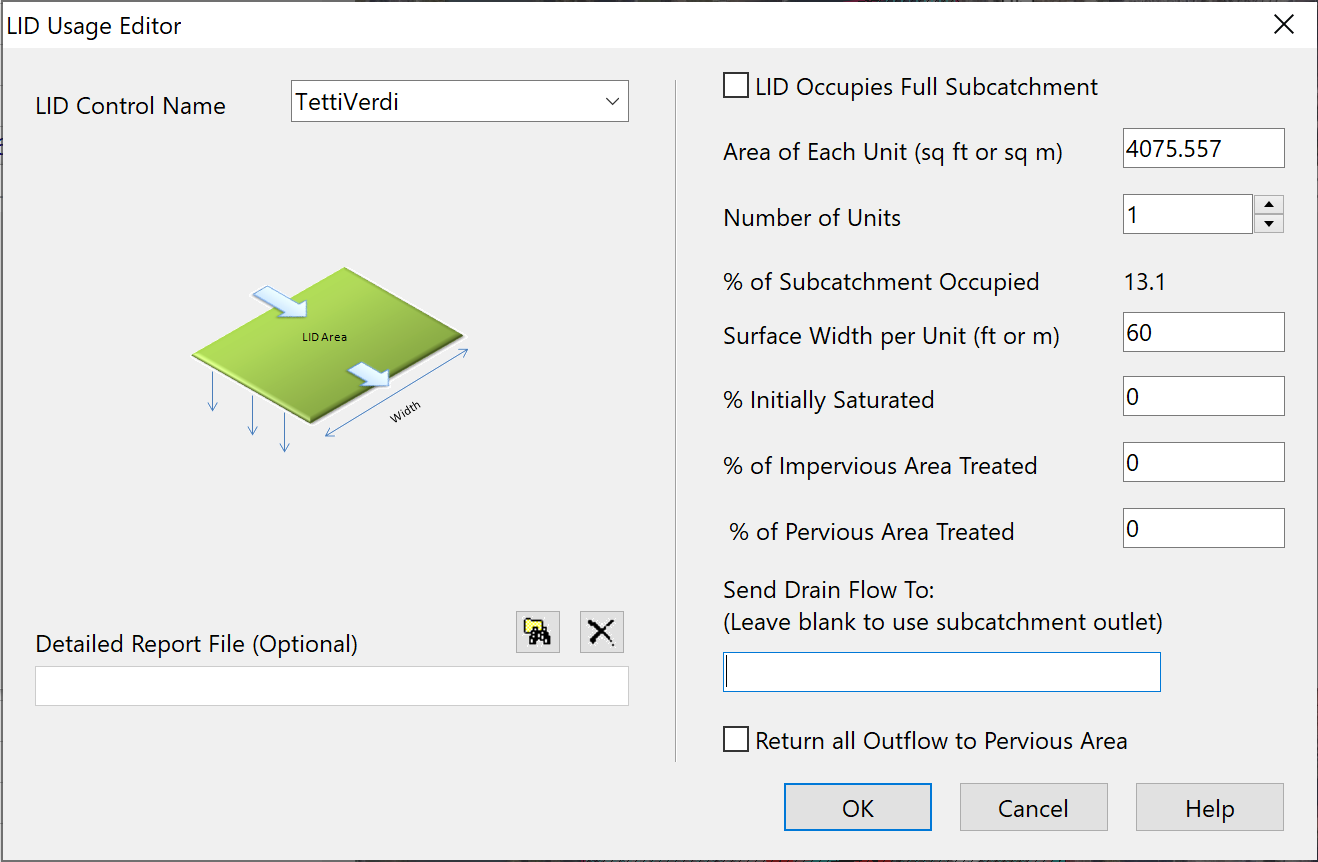
\includegraphics[height=0.42\textheight]{IMG/LID-Inflow/LID0.png}} 
        \subfloat[][\emph{Tetto verde}]{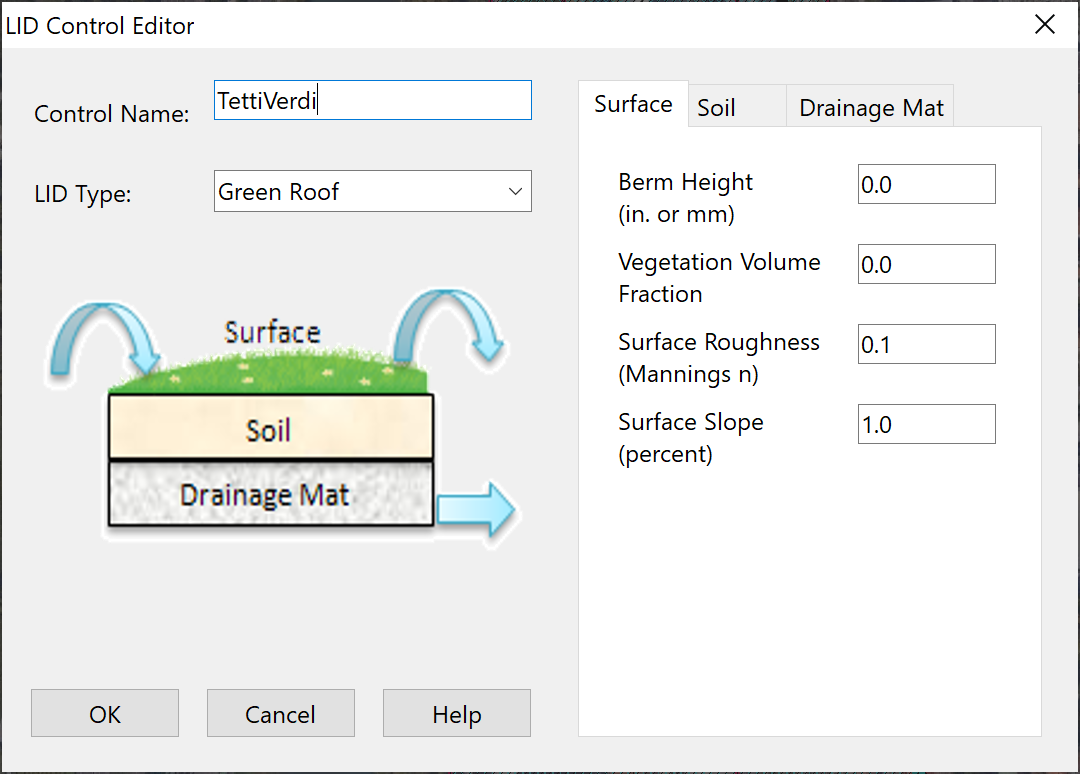
\includegraphics[height=0.42\textheight]{IMG/LID-Inflow/LID1.png}} \\
        \subfloat[][\emph{Pavimento permeabile}]{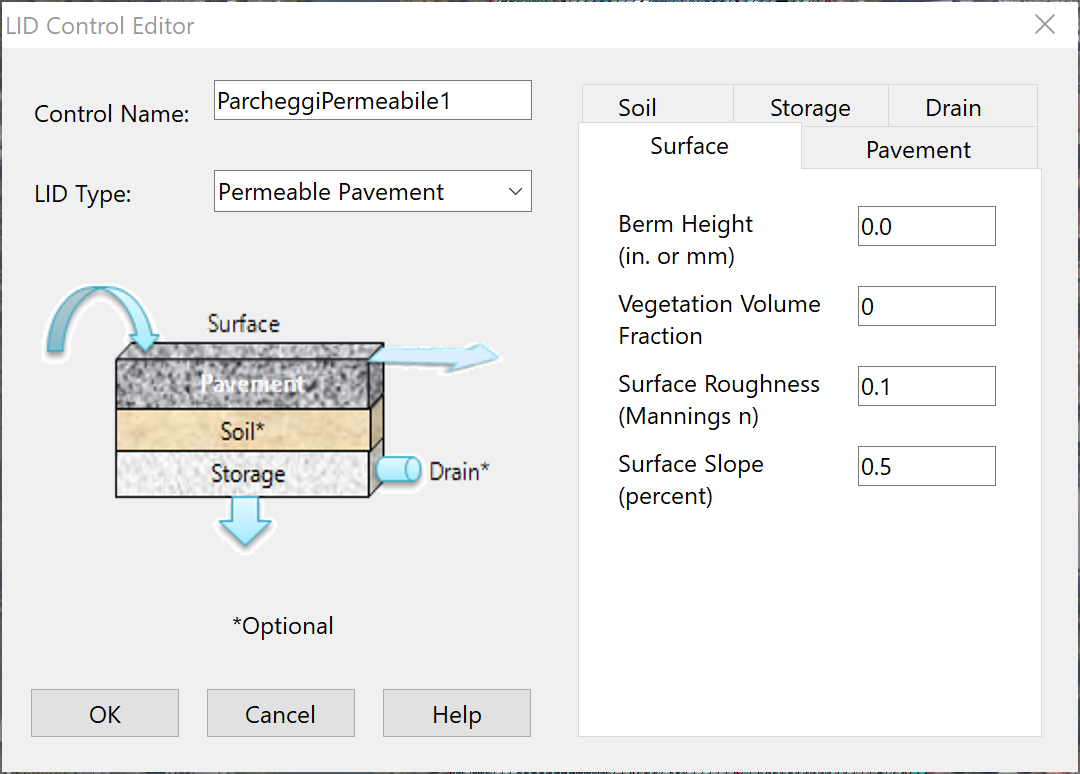
\includegraphics[height=0.42\textheight]{IMG/LID-Inflow/LID2.png}}
        \subfloat[][\emph{Celle di bio-ritenzione}]{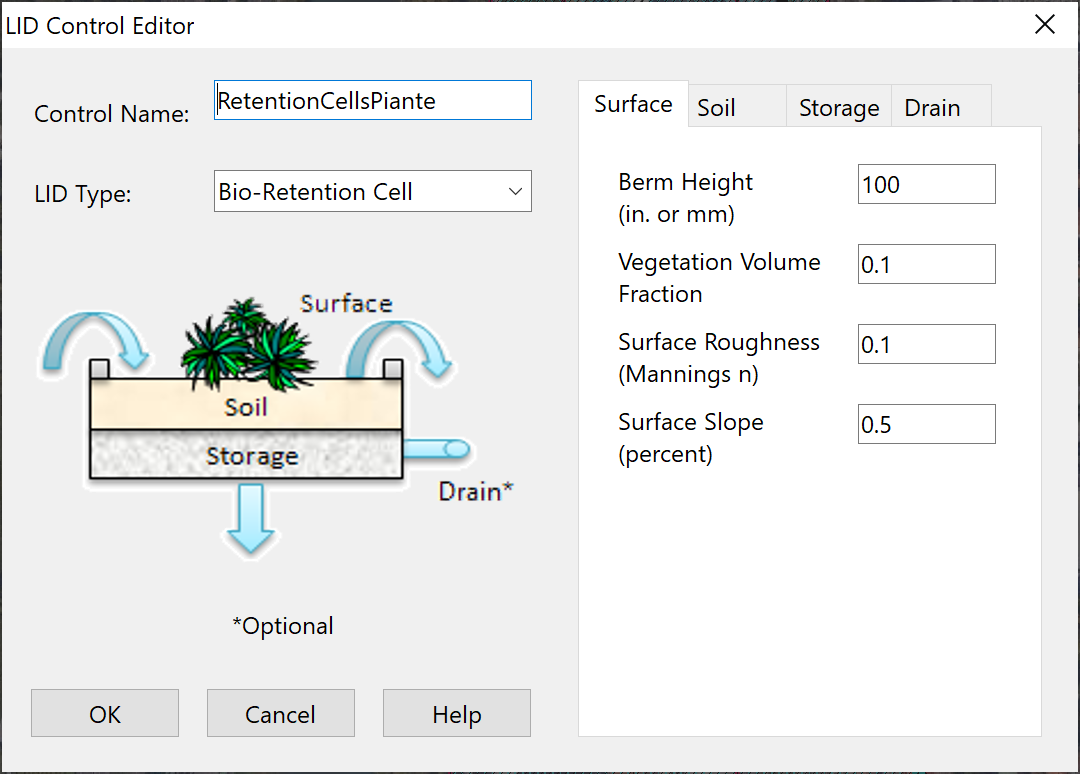
\includegraphics[height=0.42\textheight]{IMG/LID-Inflow/LID3.png}}\\
    \caption{Schermate SWMM riguardo i parametri dei LID}
    %\label{fig:ProfiliProgettoCondotte}
    \end{figure}
\end{landscape}
%
%section dentro a pagecommand manda in toc e crea il titolo
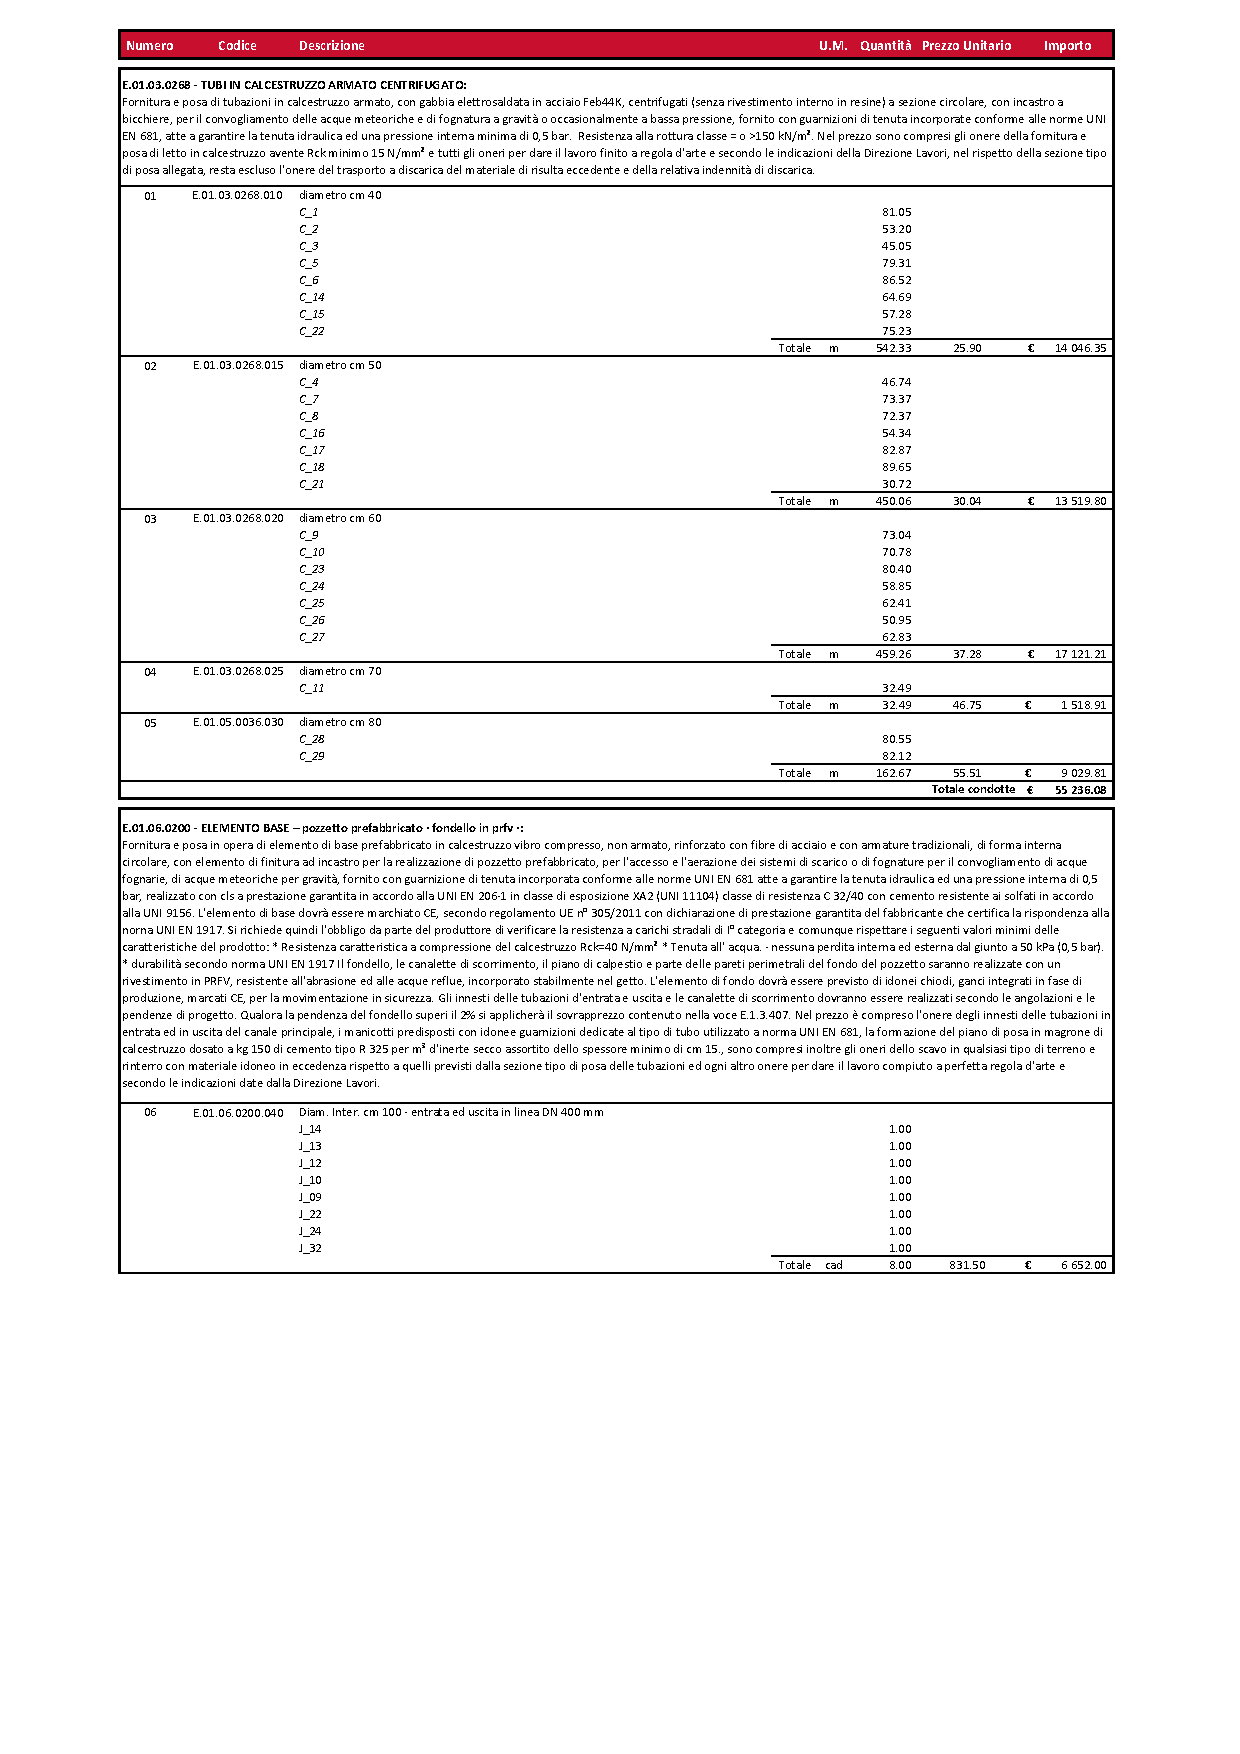
\includepdf[pages={1},pagecommand={\thispagestyle{plain},\section{Computo metrico estimativo}},offset=0 -5cm]{img/computo1.pdf}
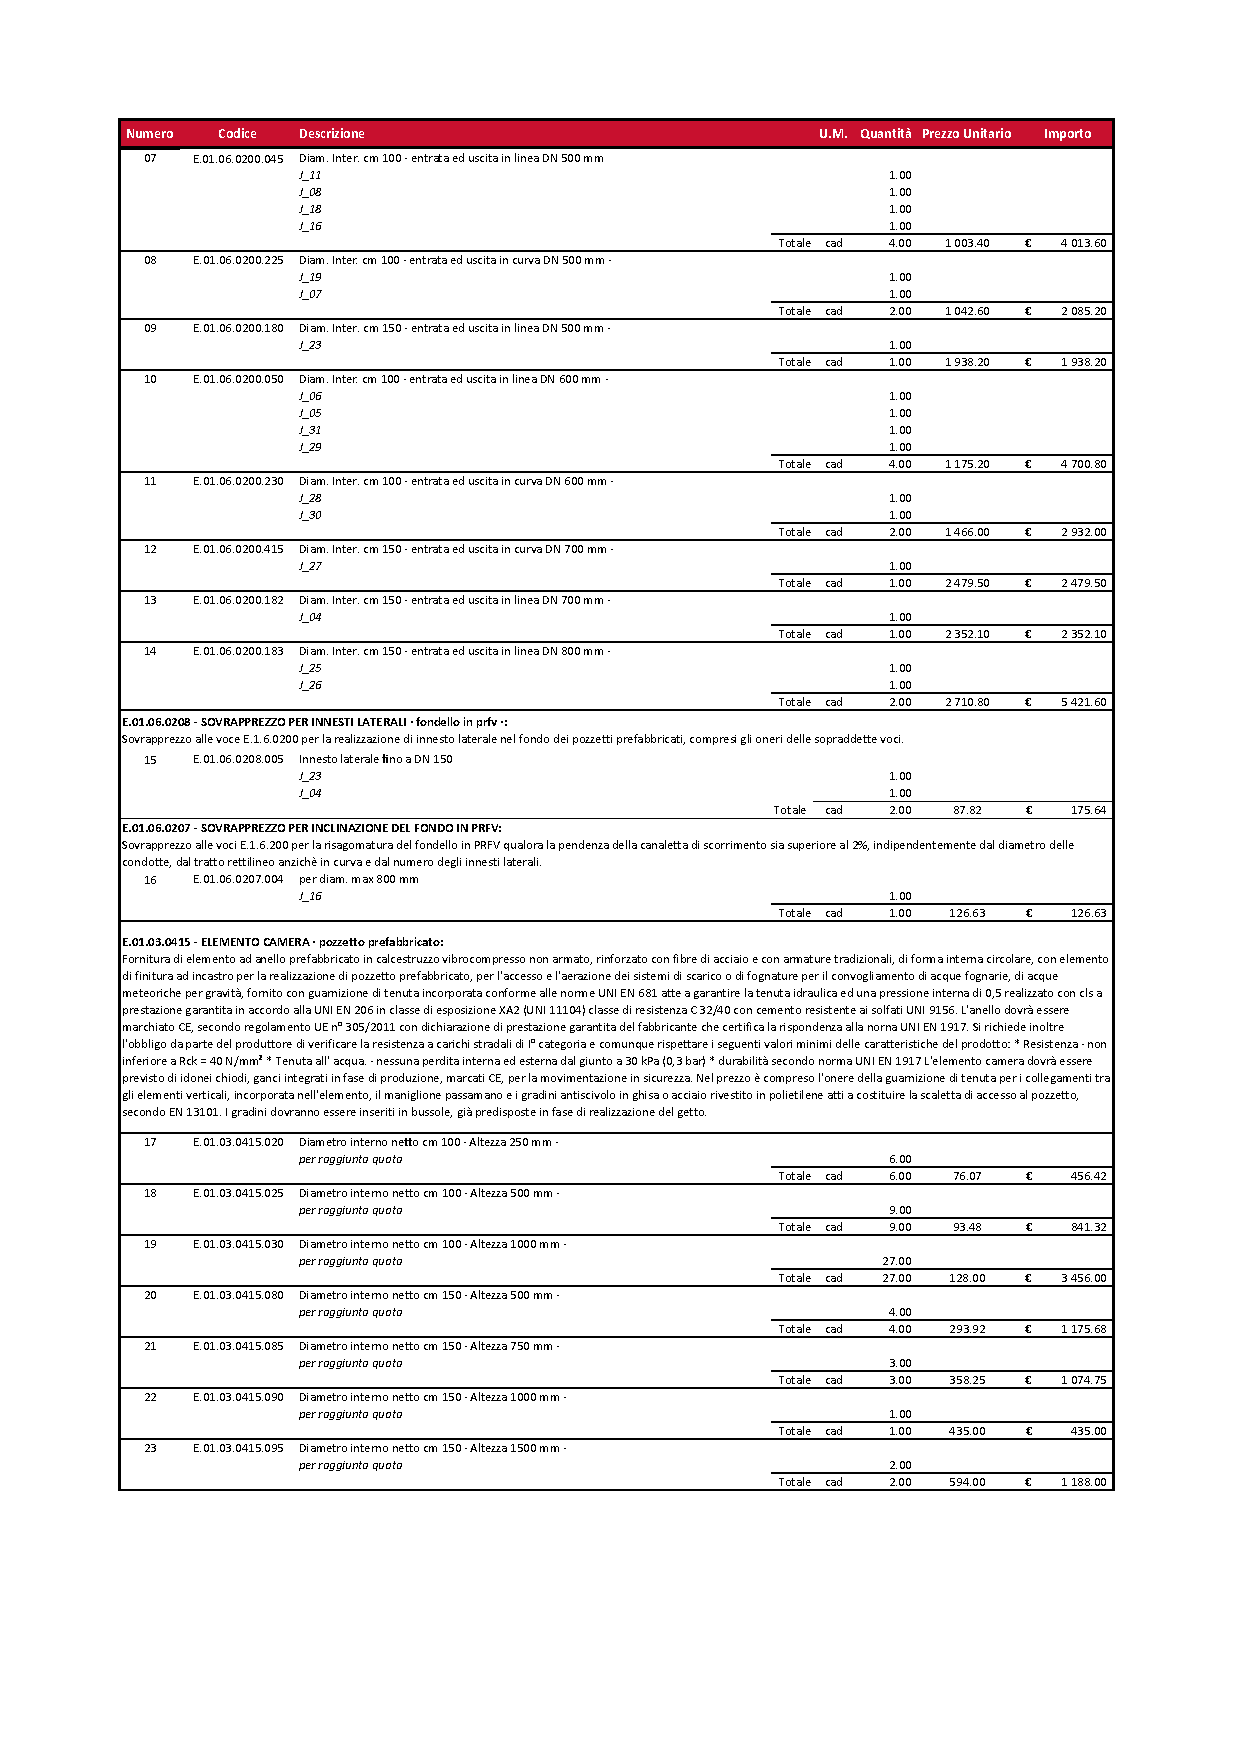
\includepdf[pages={1,2},pagecommand={\thispagestyle{plain}}]{img/computo2.pdf}


%\chapter{nome capitlo 1}
\begin{figure}[htbp]
    \centering
    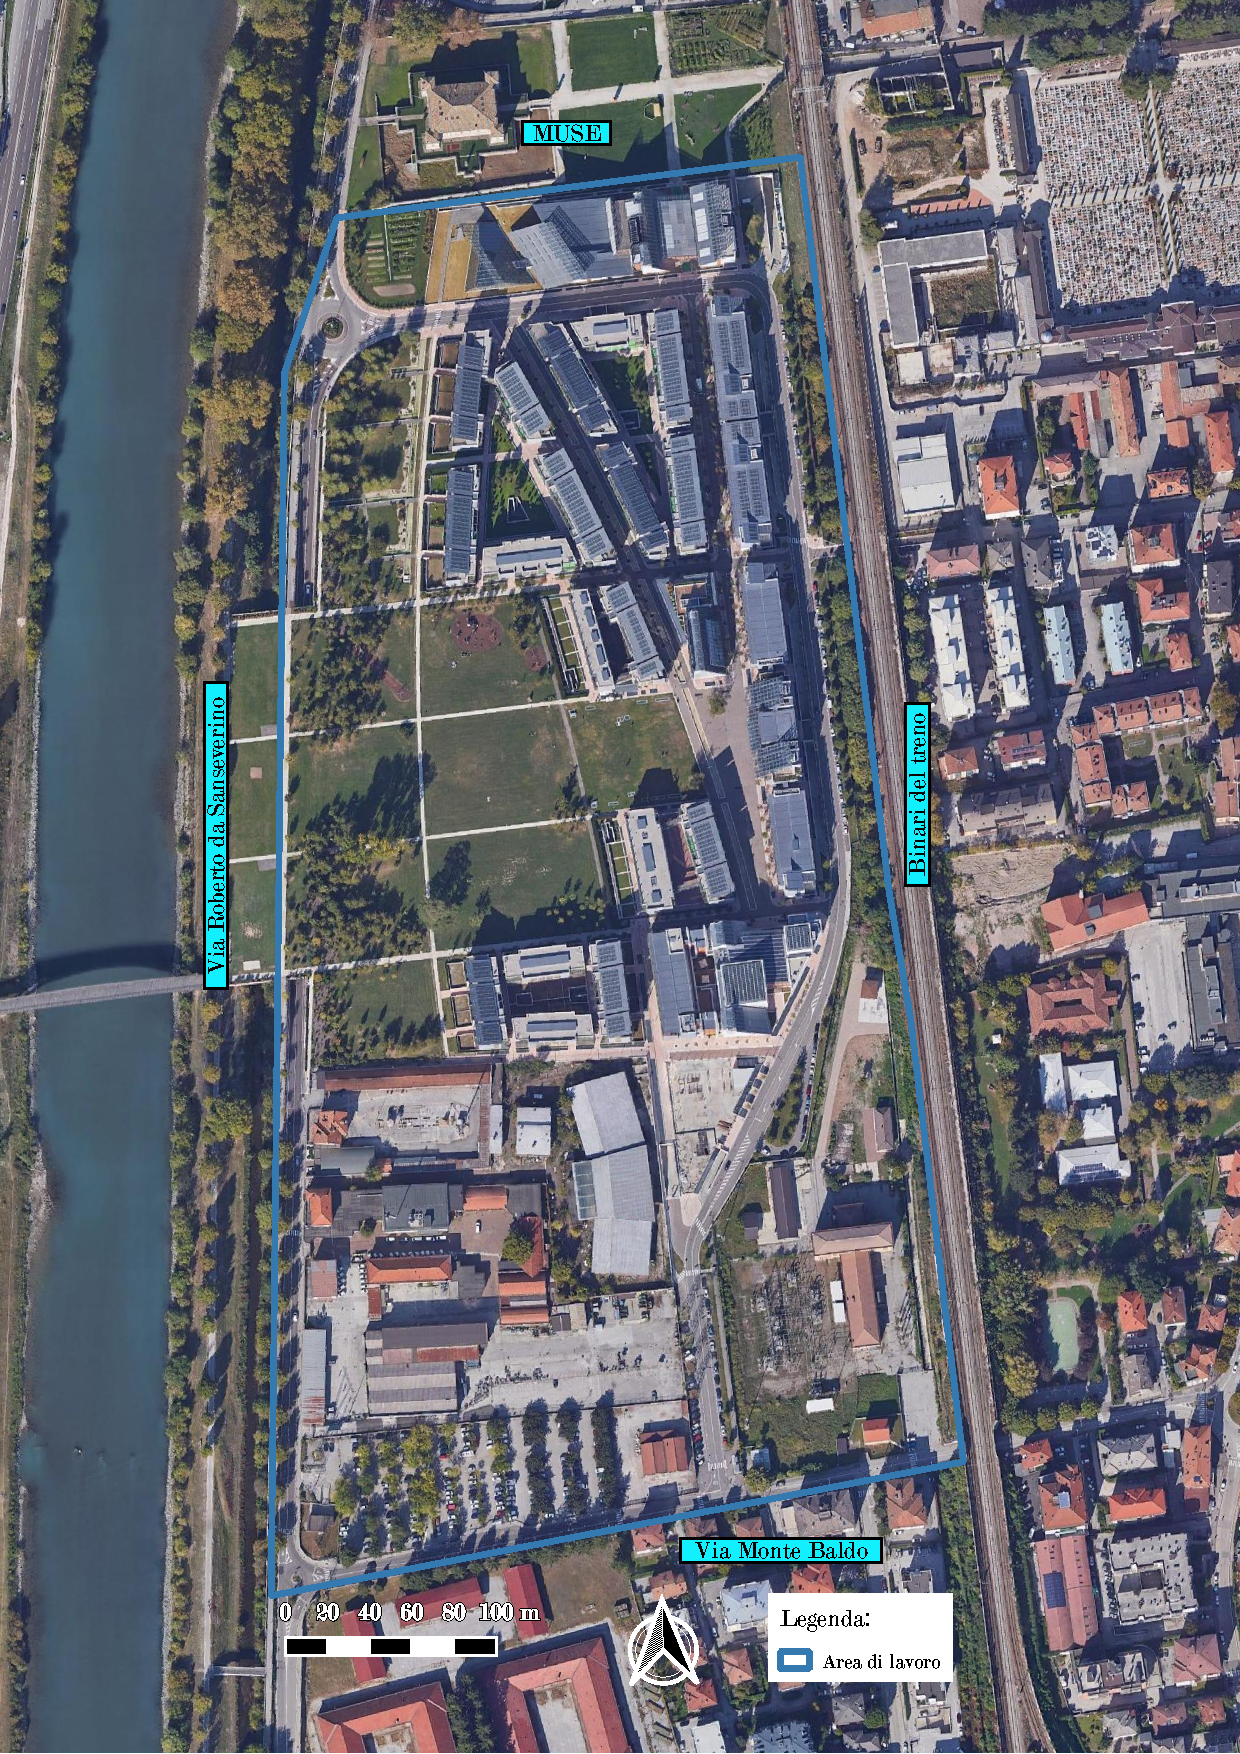
\includegraphics[trim=0cm 0cm 0cm 0cm,clip,frame,width=\textwidth]{IMG/inquadramento.pdf} 
    \caption{Inquadramento dell'area di lavoro}
    \label{fig:inquadramento}
    \end{figure}

\begin{equation}
    i = a \, t_p ^{n - 1}
\end{equation}
\begin{equation}
    CN = \frac{25400}{254 + S}
\end{equation}

\begin{equation}
    T_{\text{dry}} = \frac{3.125}{\sqrt{K_s}}
\end{equation}
Dove $T_{\text{dry}}$ sono i giorni che impiega il suolo completamente saturo a tornare secco e $K_s$ è la conduttività idraulica espressa in \si{inch\per\hour}.
\begin{equation}
    i_m = \frac{h(t_\text{fin}) - h(t_\text{in})}{\Delta t}
\end{equation}
\begin{equation}   
    h(t) = 
    \begin{cases}
        r \, a \left[ \left( \frac{t_p}{r}\right)^n - \left( \frac{t_p - t}{r}\right)^n  \right] & \text{se $t < t_p$}\\
        a \left[ r \left( \frac{t_p}{r}\right)^n + (1-r)\left( \frac{t_p - t}{1 - r}\right)^n  \right] & \text{se $t > t_p$}\\
    \end{cases}
\end{equation}
 


















\begin{landscape}
    \begin{figure}[htb]
        \centering
        \begin{tikzpicture}
            \begin{axis}[
                restrict x to domain=-0:1.5,
                height=15cm,
                width=21cm,
                grid=major,
                xlabel=Tempo trascorso dall'inizio della precipitazione \si{[\hour]},
                ylabel=Deflusso  \si{[\litre\per\second]},
                xtick = {0.5,1,1.5,2,2.5,3,3.5,4},
                %title= ,
                /pgf/number format/.cd,
                use comma,
                1000 sep={\,}
            ]
            \addplot +[mark=none,style=solid,color=red] table[x index=0,y index=1,header=false] {IMG/Total-Inflow/total_inflow_1min.txt};
            \addplot +[mark=none,style=solid,color=green!60!black] table[x index=0,y index=1,header=false] {IMG/Total-Inflow/total_inflow_2min.txt};
            \addplot +[mark=none,style=solid,color=magenta] table[x index=0,y index=1,header=false] {IMG/Total-Inflow/total_inflow_5min.txt};
            \addplot +[mark=none,style=solid,color=cyan] table[x index=0,y index=1,header=false] {IMG/Total-Inflow/total_inflow_10min.txt};
            \addplot +[mark=none,style=solid,color=orange] table[x index=0,y index=1,header=false] {IMG/Total-Inflow/total_inflow_15min.txt};
            \addplot +[mark=none,style=solid,color=teal] table[x index=0,y index=1,header=false] {IMG/Total-Inflow/total_inflow_30min.txt};
            \addplot +[mark=none,style=solid,color=violet] table[x index=0,y index=1,header=false] {IMG/Total-Inflow/total_inflow_45min.txt};
            \legend{1 min,2 min,5 min,10 min,15 min,30 min,45 min}    
            \end{axis}
        \end{tikzpicture}
        \caption{Deflusso del bacino}
        \label{fig:Ietogrammi}
    \end{figure}
\end{landscape}

\begin{landscape}
    \begin{figure}[htb]
        \centering
        \begin{tikzpicture}
            \begin{axis}[
                restrict x to domain=-0:4,
                height=15cm,
                width=21cm,
                grid=major,
                xlabel=Tempo trascorso dall'inizio della precipitazione \si{[\hour]},
                ylabel=Total Inflow  \si{[\litre\per\second]},
                xtick = {0.5,1,1.5,2,2.5,3,3.5,4},
                %title= ,
                /pgf/number format/.cd,
                use comma,
                1000 sep={\,}
            ]
            \addplot +[mark=none,style=solid,color=red] table[x index=0,y index=1,header=false] {IMG/Total-Inflow/total_inflow_5min_Chicago_25anni.txt};
            \end{axis}
        \end{tikzpicture}
        \caption{Andamento dello sforzo assiale agente sul pilastro P27 in funzione dell'altezza}
        \label{fig:IetogrammaFinale}
    \end{figure}   
\end{landscape}
%\chapter{Rete di smaltimento delle acque meteoriche allo stato di progetto (con presenza
della rete di drenaggio)} \label{cap:ProgettoRete}
Analizzato quindi il deflusso dei sottobacini presenti nell'area di lavoro, si passa ora alla fase progettuale della rete di drenaggio. 
Tale progettazione sarà suddivisa in tre fasi principali in quanto si è voluto studiare tre casistiche di intervento: una rete di drenaggio composta da sole condotte e tombini, la precedente rete con l'aggiunta di sistemi di laminazione puntuale ed infine l'ulteriore aggiunta di sistemi di laminazione diffusi.

Dato il procedimento iterativo che compone ciascuna fase e il relativo aggiustamento dimensionale delle condotte (dovuto ad esempio  a sottobacini troppo piccoli e verifiche non soddisfatte, ecc) oppure della ri-progettazione della rete con solo i sistemi diffusi (per ottimizzare la dimensione delle condotte) e successiva aggiunta dei sistemi puntuali, si è voluto riportare in questo capitolo solo i risultati delle tre fasi principali sopra descritte e di  non riportare invece le fasi intermedie. %nell'appendice \ref{appendix:FasiIntermedie} a pagina \pageref{appendix:FasiIntermedie}. 

Di seguito verranno dapprima riportati i passaggi che contraddistinguono il dimensionamento e la verifica delle condotte in comune di ciascuna fase, per poi concentrarsi su ciascuna casistica riportando i risultati in forma per lo più tabellare o grafica.

\section{Procedimento per il progetto e verifica}
Data la necessità di conoscere il volume di riempimento delle condotte, la presenza di rigurgito o di moto in pressione è necessario cambiare le modalità di calcolo per la risoluzione della rete.
Nelle ipotesi di moto vario a superficie libera monodimensionale e con condotte di piccola pendenza, gradualmente variato e con fluido incomprimibile si utilizza ora il metodo dell'\emph{Onda Dinamica} che consiste nel considerare tutti i termini dell'equazione di De Saint Venant \ref{eq:saintvenant} relativa alla conservazione della quantità di moto, senza perciò trascurare quelli relativi al gradiente di pressione (come nel metodo dell'\emph{Onda Cinematica} visto prima in cui si era posto $S_0 = S_f$) e i termini inerziali. 
\begin{equation}
    \label{eq:saintvenant}
    \frac{\partial Q}{\partial t} + \frac{\partial}{\partial x} \left( \frac{Q^2}{A} \right) + g A \frac{\partial y}{\partial x} - g A (S_0 - S_f) = 0
 \end{equation}

\subsection{Profondità scavo}
Una volta scelto il percorso delle condotte e dei relativi tombini di collegamento, si deve fare in modo di allineare ciascuna di esse al cielo: 
questo per consuetudine italiana in cui si vuole avere più facilità di manutenzione e di posa degli strati in sommità delle condotte. 
Occorre quindi ipotizzare una pendenza delle condotte $i_g^{prog}$ di primo tentativo e successivamente calcolare la profondità di scavo (\emph{Max Depth}) data dalla differenza tra la quota del terreno e la quota di fondo.
La quota del terreno la si ottiene dai dati altimetrici dell'area (estratti usando QGIS), mentre la quota di fondo è data dalla somma, da valle a monte, dei dislivelli $\Delta h = i_g^{prog} \cdot L_{\text{condotta}}$ di ciascun tratto, partendo dalla quota nota dei recapiti finali (chiamati R1, R2, R3 nelle tabelle e nelle figure che seguiranno d'ora in poi).

Si ottiene così per ogni tratto una \emph{Max Depth} che deve essere
\begin{equation}
    \SI{1.5}{\metre} \lessapprox Max Depth \lessapprox\SI{6.5}{\metre}\quad ,
\end{equation} 
in modo di avere da un lato un ricoprimento minimo delle condotte tale che non si danneggino con il carico di veicoli, persone o intemperie;  dall'altro un ricoprimento contenuto da non avere costi di scavo troppo elevati. 
Per stare all'interno di tale intervallo si va ad agire sulla pendenza di progetto delle condotte o, eventualmente, su sistemi di rinforzo delle stesse.
\subsection{Diametro}
\begin{figure}[H]
    \centering
    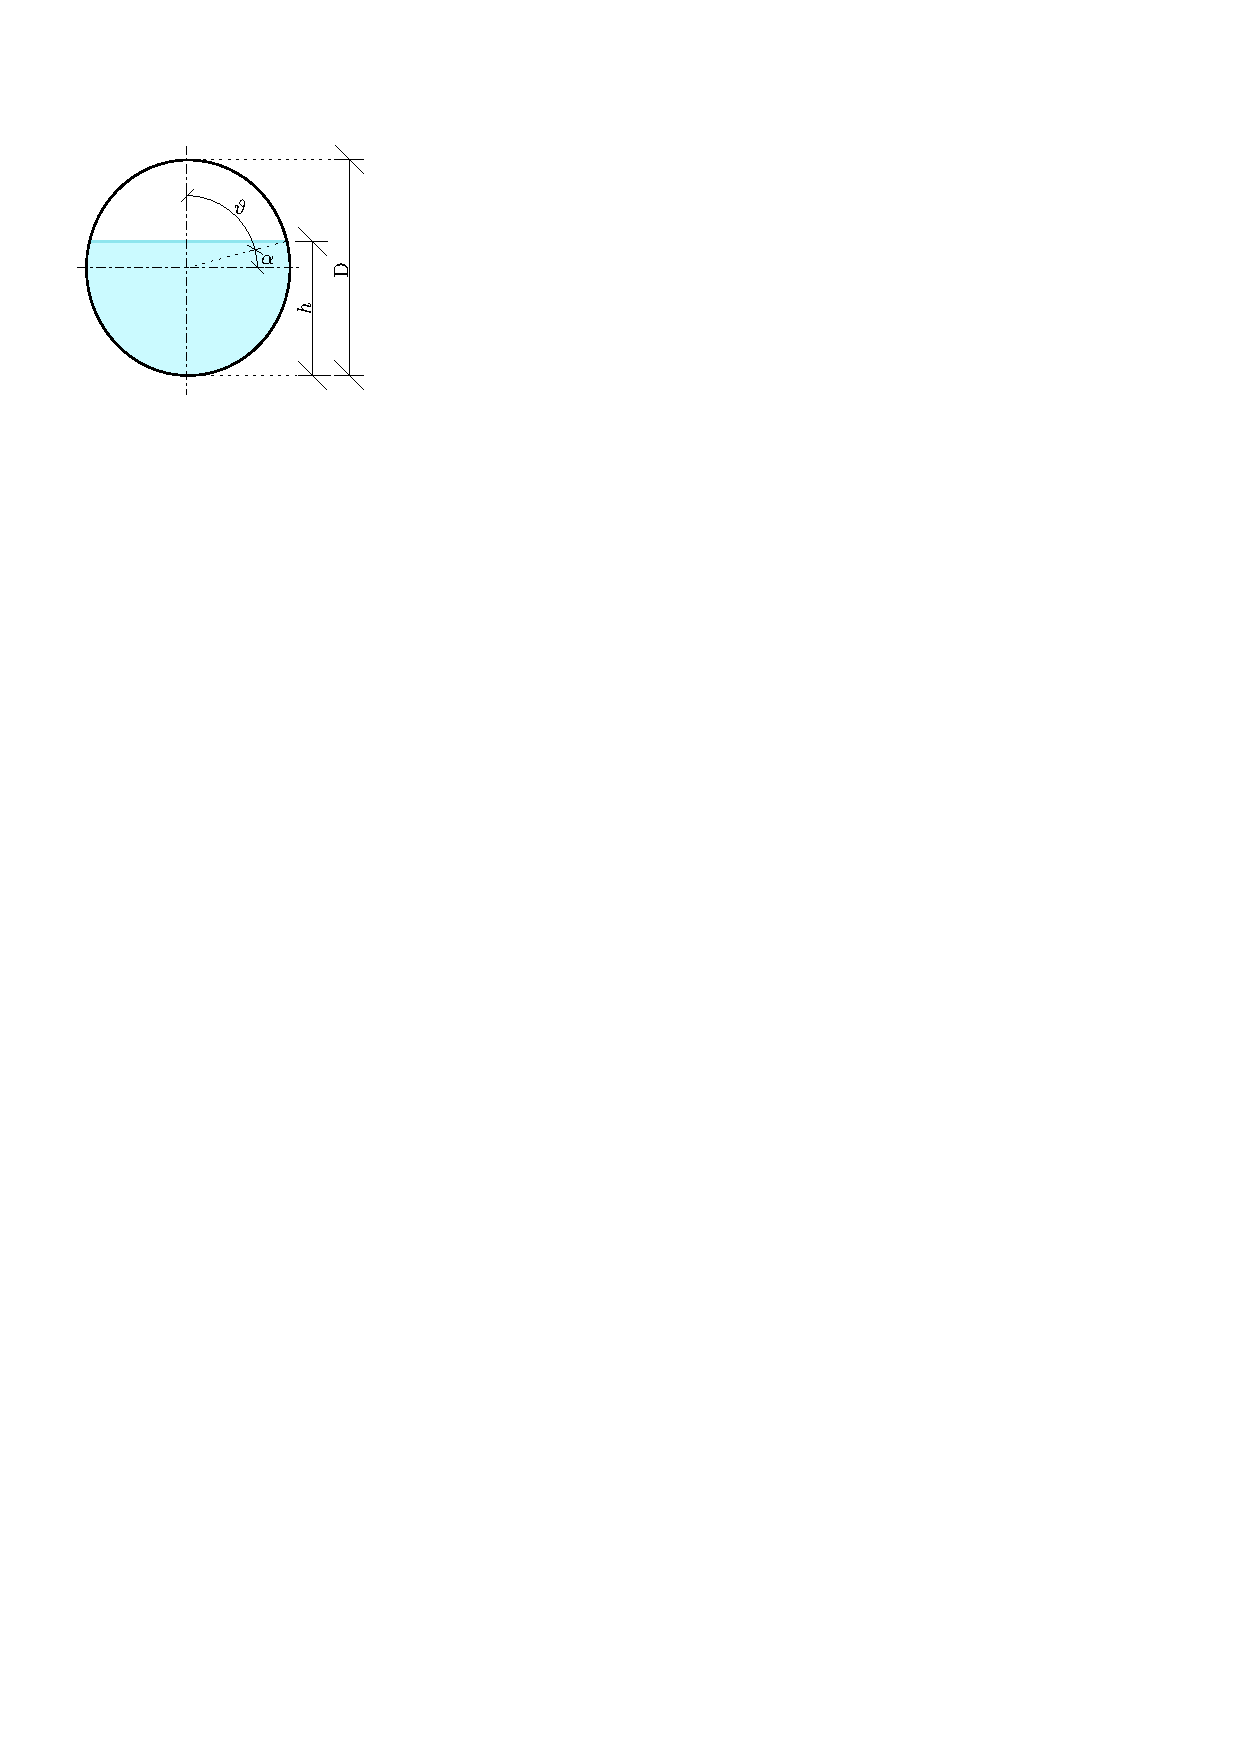
\includegraphics[]{IMG/RiempimentoCondotta.pdf}
\end{figure}
Con le ipotesi di moto sopra dette, si deve progettare la dimensione delle condotte facendo in modo di rispettare il loro riempimento così da rimanere all'interno delle ipotesi. 
Per questo si è imposto un riempimento ideale $\hat{\beta}$ del \SI{75}{\percent}
\begin{equation}
    \hat{\beta} = \frac{h}{D} = \SI{0.75}{} \quad .
\end{equation}

Dalla formula di Chézy, con la formulazione di Gauckler-Strickler, applicata al caso di condotte a sezione circolare e in riferimento alla nomenclatura di figura sopra, si ha tale legge che esprime la portata in funzione del riempimento:
\begin{equation}
    Q(\beta) 
    = A(\beta) \, k_s \, R^{\tfrac{2}{3}} \, i^{\tfrac{1}{2}} 
    = \frac{ D \, k_s \, f(\beta)^{\tfrac{5}{3}} \, i^{\tfrac{1}{2}} }{ 2^{\tfrac{13}{3}} \, g(\beta)^{\tfrac{2}{3}} }
\end{equation}
dove 
\begin{align}
    f(\beta) &= \pi - 2 \alpha - 2 (1 - 2 \beta) \cos(\alpha) \\
    g(\beta) &= \pi - 2 \alpha \\
    \alpha &= \arcsin(1 - 2 \beta)
\end{align}
e dalla quale si può ricavare il diametro minimo per il riempimento $\beta = \hat{\beta}$ fissato, avendo nota la portata $Q$ pari al deflusso a monte di tale condotta:
\begin{equation}
    D_{prog}(\hat{\beta}) = \frac{ 2^{\tfrac{13}{8}} \, g(\hat{\beta})^{\tfrac{1}{4}} }{     K_S^{\tfrac{3}{8}} \, f(\hat{\beta})^{\tfrac{5}{8}} } \frac{Q^{\tfrac{3}{8}}}{i^{\tfrac{3}{16}}} \quad .
\end{equation} 

Da tale diametro minimo se ne va a scegliere uno di sezione immediatamente superiore -- o al più di poco inferiore, a causa delle verifiche di riempimento nel capitolo successivo -- disponibile commercialmente.

Infine si calcola per ogni tratto la differenza di dimensione tra la condotta con diametro maggiore e tutte le altre, in modo da inserirle in SWMM e ottenere l'allineamento al cielo.

\subsection{Verifiche alle condotte}
Si deve ora verificare che le ipotesi fatte in fase progettuale siano state rispettate. 
Riguardo al riempimento ideale $\hat \beta$ imposto si deve controllare che il riempimento della condotta $\beta_\text{cond.}$ risulti 
\begin{equation}
    \SI{50}{\percent} \lessapprox \beta_\text{cond.} \lessapprox\SI{75}{\percent} \quad .
\end{equation}

Seguendo le indicazioni del Consiglio Superiore dei Lavori Pubblici la velocità dell'acqua all'interno delle condotte deve essere:
\begin{equation}
    \SI{0.5}{\metre\per\second} < V <  \SI{5}{\metre\per\second} \quad .
\end{equation}
Questo per non avere velocità troppo basse tali da formare dei sedimenti né velocità troppo elevate tali da danneggiare il materiale stesso delle condotte.
In realtà, per verificare che non si creino sedimenti nei periodi di non-precipitazione e rispettare il cosiddetto criterio di autopulizia, si è utilizzato anche un altro metodo che fa riferimento ad una tensione tangenziale al fondo $\tau$ minima oppure ad una pendenza del fondo (o idraulica) $i_f$ massima. 
Ovvero si deve avere:
\begin{equation}
    \label{eq:tau}
    \tau = \gamma \, R_H \, i_g > \SI{2}{\pascal}
\end{equation}
dove $\gamma$ è il peso specifico dell'acqua pari a \SI{1000}{\newton\per\metre\cubed}, $R_H$ è il raggio idraulico calcolato come rapporto tra area e perimetro bagnati, mentre $i_g$ è la pendenza geometrica delle condotte.  
\begin{align}
    R_H &= \frac{D}{4} \, \frac{1 - \sin(\vartheta)}{\vartheta} \\
    \vartheta &= 2 \, \arccos(1 - \beta_\text{cond.})
\end{align}
O analogamente
\begin{equation}
    i_g > i_f  
\end{equation}
in cui dalla \ref{eq:tau} si ha 
\begin{equation}
    i_f = \frac{\tau}{R_H \, \gamma} \biggr|_{\tau=\SI{2}{\pascal}}
\end{equation}    
mentre $i_g$ rimane la pendenza geometrica delle condotte, la quale deve essere comunque almeno del \SI{0.5}{\percent}.






\section{Progetto}
\label{cap:ProgettoCondotte}
Il progetto della rete di drenaggio prevede tre rami principali ciascuno composto da altrettanti recapiti finali affluenti al canale Adigetto. 
I rami principali delle condotte, visibili nel dettaglio in figura \ref{fig:Condotte} nella fase progettuale finale, sono posti a nord, centro e sud dell'area di studio in concomitanza dei tre recapiti $R1$, $R2$, $R3$ posti a quota prefissata di \SI{184.00}{}, \SI{183.70}{} e \SI{183.50}{\metre}.
\begin{figure}[p]
    \centering
    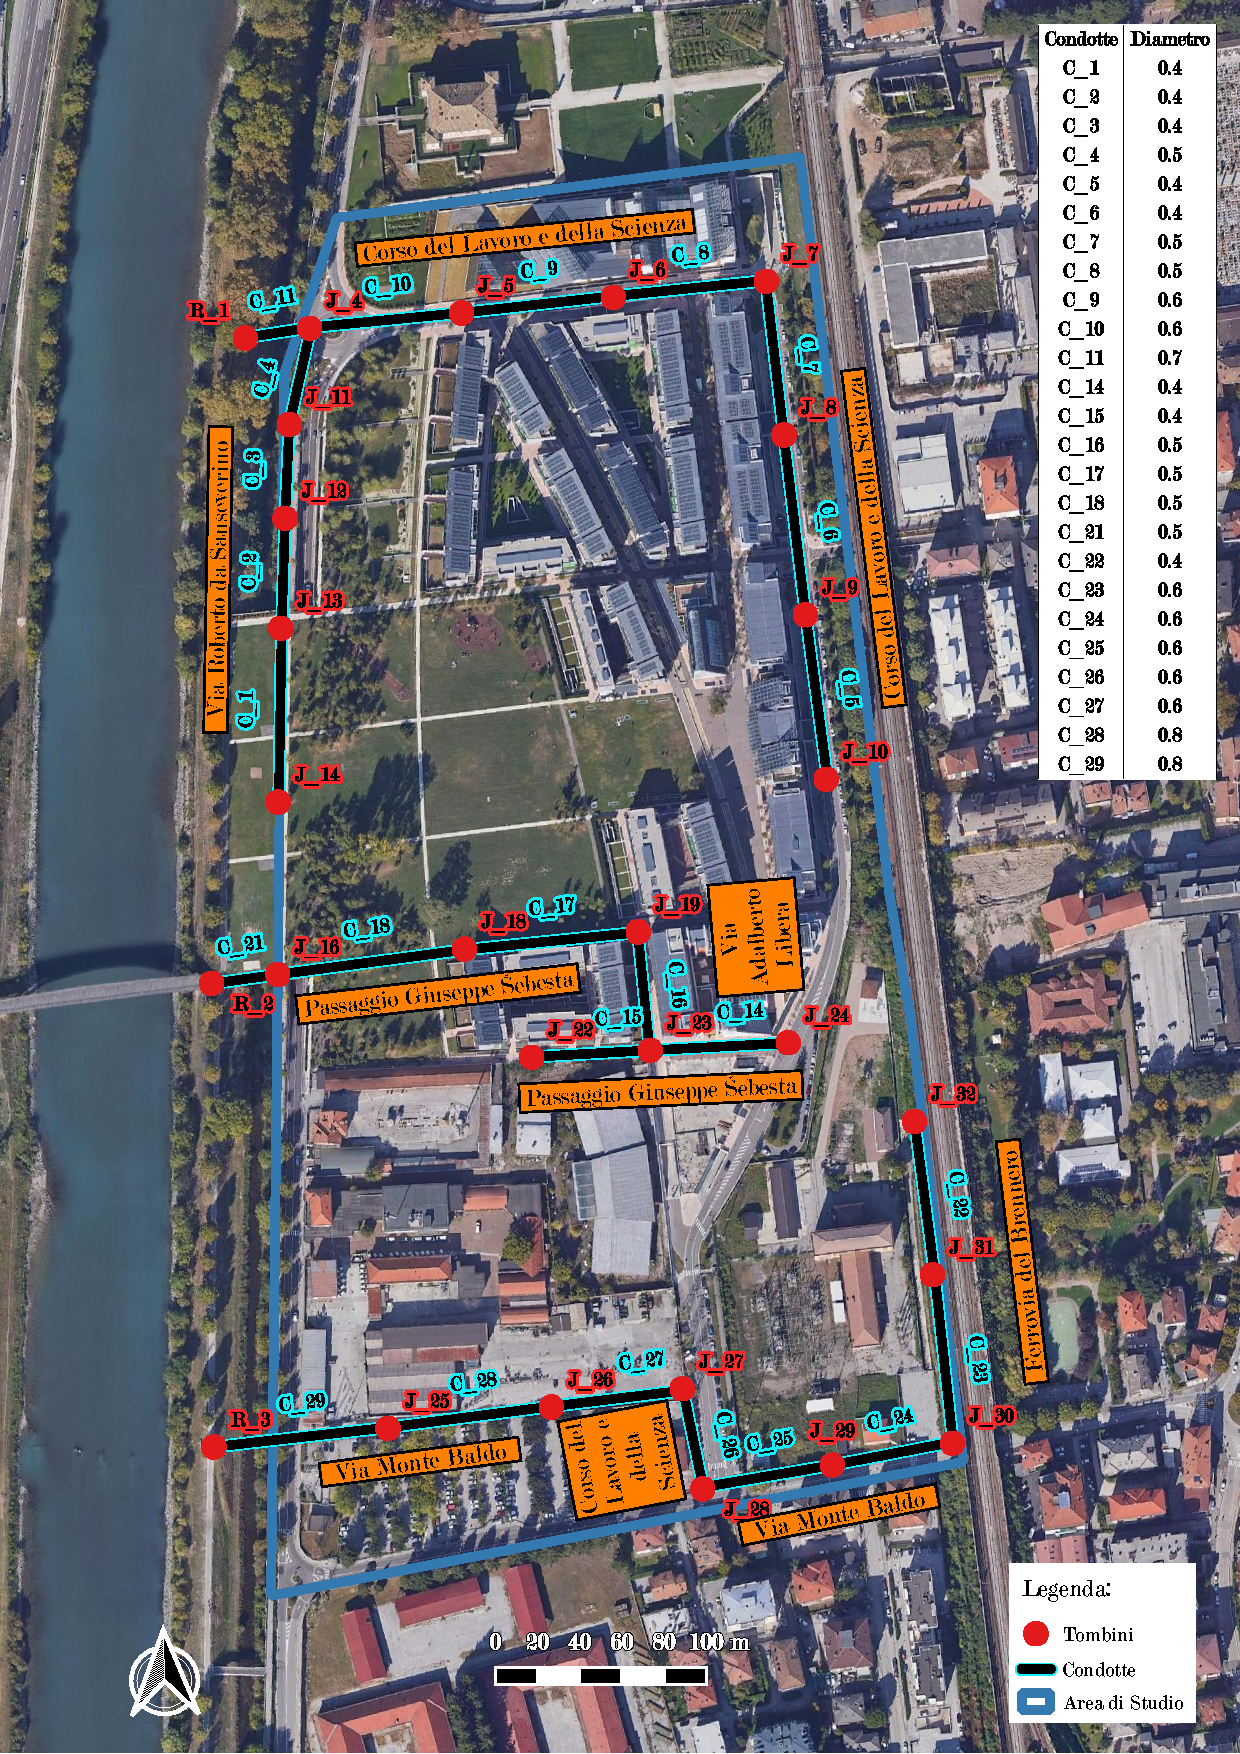
\includegraphics[trim=0cm 0cm 0cm 0cm,clip,frame,width=0.9\textwidth]{IMG/Nomenclatura_condotte.pdf} 
    \caption{Posizionamento e nomenclatura della rete di drenaggio con indicazione del deflusso dei sottobacini}
    \label{fig:Condotte}
\end{figure}

Il percorso delle reti cerca di sovrapporsi a strade o vicoli pre-esistenti in modo da non aumentare l'impatto ambientale e visivo. 
Cerca inoltre di attraversare ogni sottobacino per confluire ad ognuno il deflusso in un rispettivo tombino, idealmente a monte della condotta. 
In questo modo si riesce a dimensionare con maggiore efficacia le tubazioni. 
In aggiunta le condotte devono essere interrotte da un tombino d'ispezione e non divenire più lunghe di \SI{100}{\metre}.

Per tutte le componenti della rete è stato usato calcestruzzo armato senza nessun particolare rivestimento per cui, avendo condotte circolari con pareti non perfettamente lisce, si è scelto un coefficiente di Gauckler-Strickler $k_s$ pari a \SI{80}{\metre\tothe{1/3}\per\second} -- equivalente ad un numero di Manning $n$ di \SI{0.0125}{\metre\tothe{1/3}\second}, avendo usato il software SWMM di concezione anglosassone.

Il procedimento descritto nel paragrafo precedente è alla base dei dati tabulari di seguito esposti.  
Nella tabella \ref{tab:Nodi_nodes-mod} è riportata la profondità di scavo in base alla pendenza scelta delle condotte. 
Nella tabella successiva si ha il calcolo del diametro di progetto e la relativa scelta del diametro commerciale, facendo attenzione alle verifiche di riempimento e di velocità visibili invece nell'ultima tabella a seguire.

Nel tombino $J13$ non riuscendo a rispettare la profondità di scavo minima di \SI{1.5}{\metre}, ma essendo invece di \SI{0.85}{\metre}, si prevede una soletta armata sopra il tombino e lungo parte delle due condotte ad esso collegate per evitare la rottura a taglio del calcestruzzo dovuto a carichi sovrastanti. 

Nel caso delle condotte 18 e 21 si è scelto un diametro commerciale maggiore del dovuto per non avere scalini con le condotte a monte nei quali si accumulerebbero detriti. 

In figura \ref{fig:ProfiliProgettoCondotte} a pagina \pageref{fig:ProfiliProgettoCondotte} è mostrato l'andamento del pelo libero dell'acqua all'interno delle condotte nel momento di massimo picco.

Come si nota dalla figura \ref{fig:Condotte} alcuni sottobacini sono stati in realtà considerati uniti, facendo convogliare il deflusso nello stesso tombino.
Questo perché con la disposizione iniziale non si soddisfava la verifica del riempimento minimo.
%La disposizione iniziale si può vedere in appendice \ref{appendix:FasiIntermedie} nella fi e LE TABELLE SBAGLIATE a pagina TOT.

\TabellaNodi{Profondità di scavo dei tombini e pendenza progettuale delle condotte -- Progetto base con solo condotte}{tab:Nodi_nodes-mod}{IMG/Nodi-nodes-mod.tex}
\TabellaDiametriCondotte{Diametro commerciale e offset per l'allineamento al cielo -- Progetto base con solo condotte}{tab:Diametri_conduct-mod}{IMG/Diametri-conduct-mod.tex}
\TabellaVerificheLinkFLow{Verifiche massima velocità, riempimento e criterio di autopulizia -- Progetto base con solo condotte}{tab:LinkFlow_Verifiche-MOD}{IMG/LinkFlow-Verifiche-MOD.tex}
\begin{figure}[p]
    \centering
    % \subfloat[][\emph{Campata 1\label{fig:MomentiUnitariA}}]
    \subfloat[][\emph{Ramo di condotte tra il recapito finale 1 ed il tombino $J10$}]{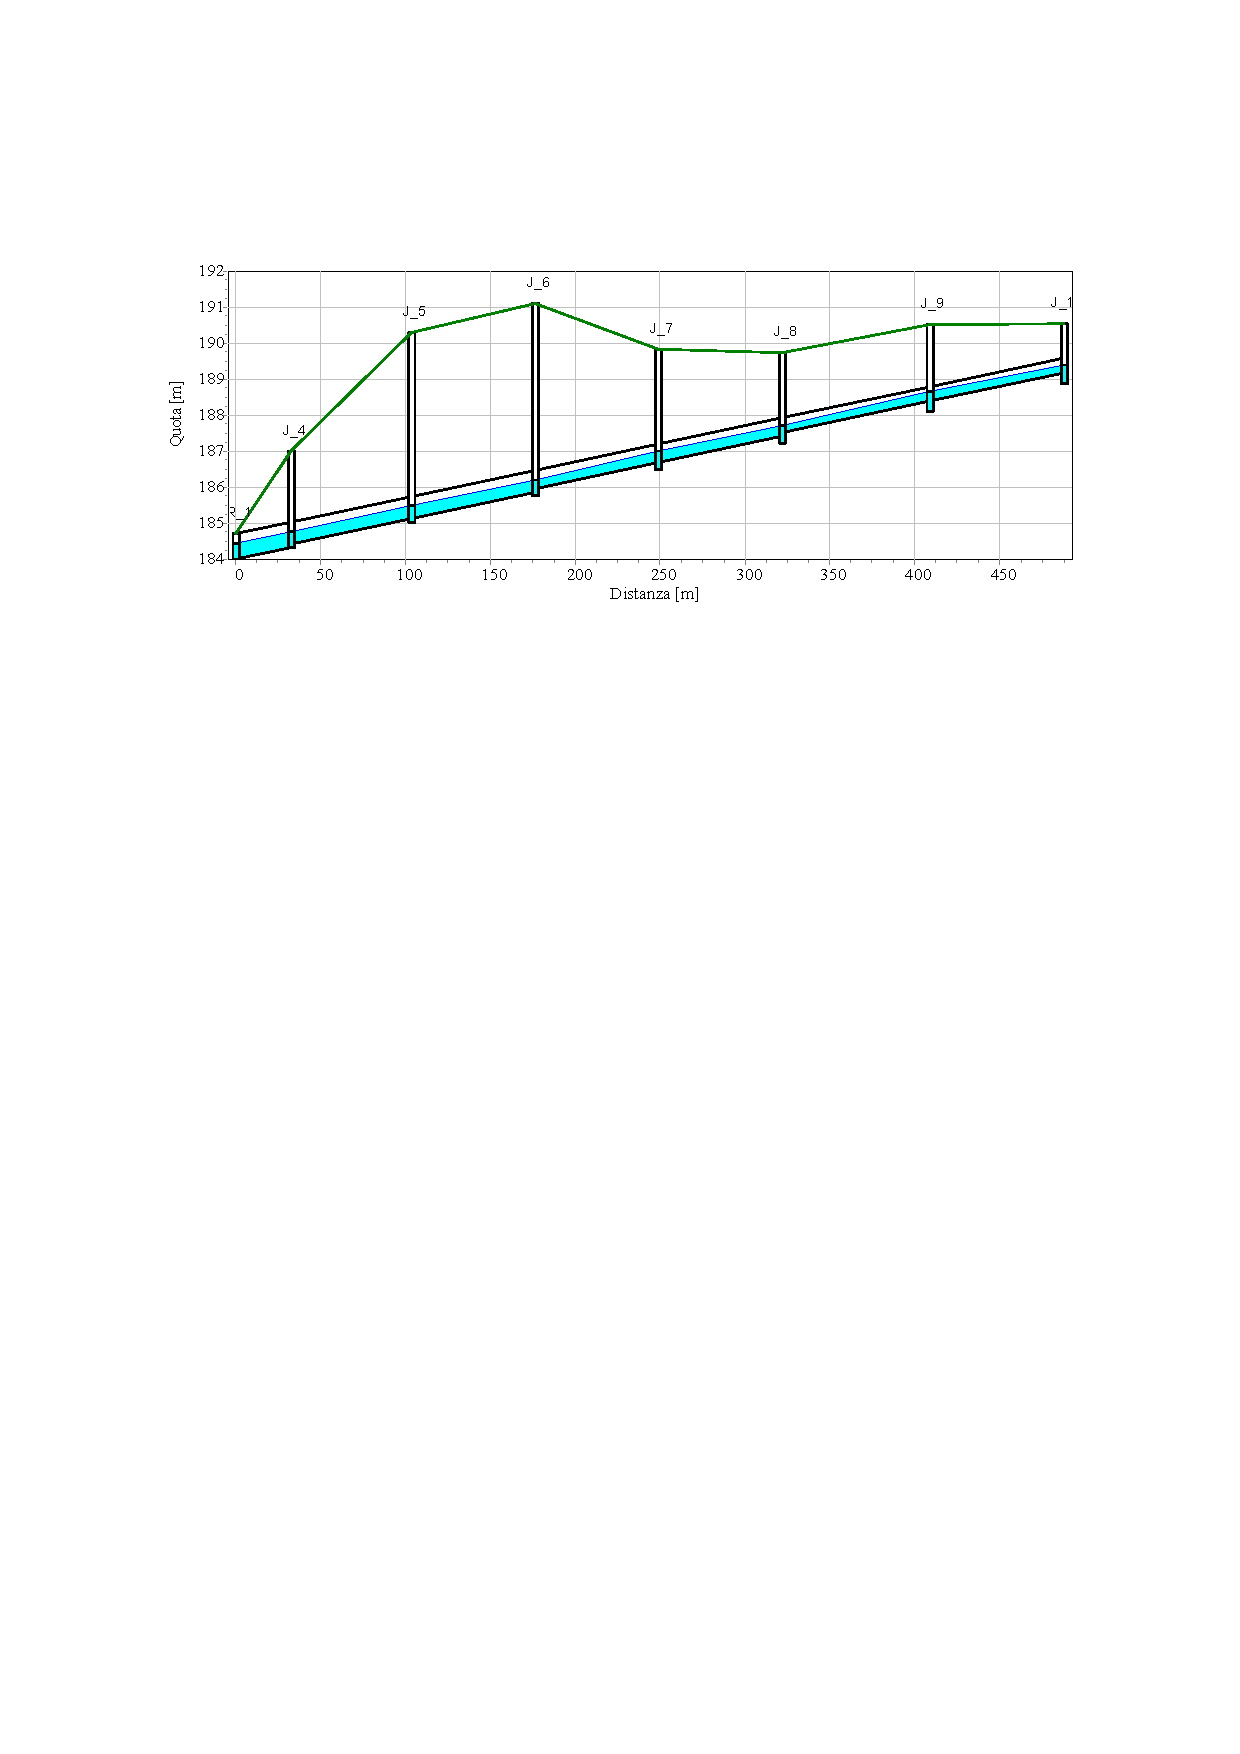
\includegraphics[width=\textwidth]{IMG/ProgettoCondotte_profiloA.pdf}} \\
    \subfloat[][\emph{Ramo di condotte tra il recapito finale 2 ed il tombino $J24$}]{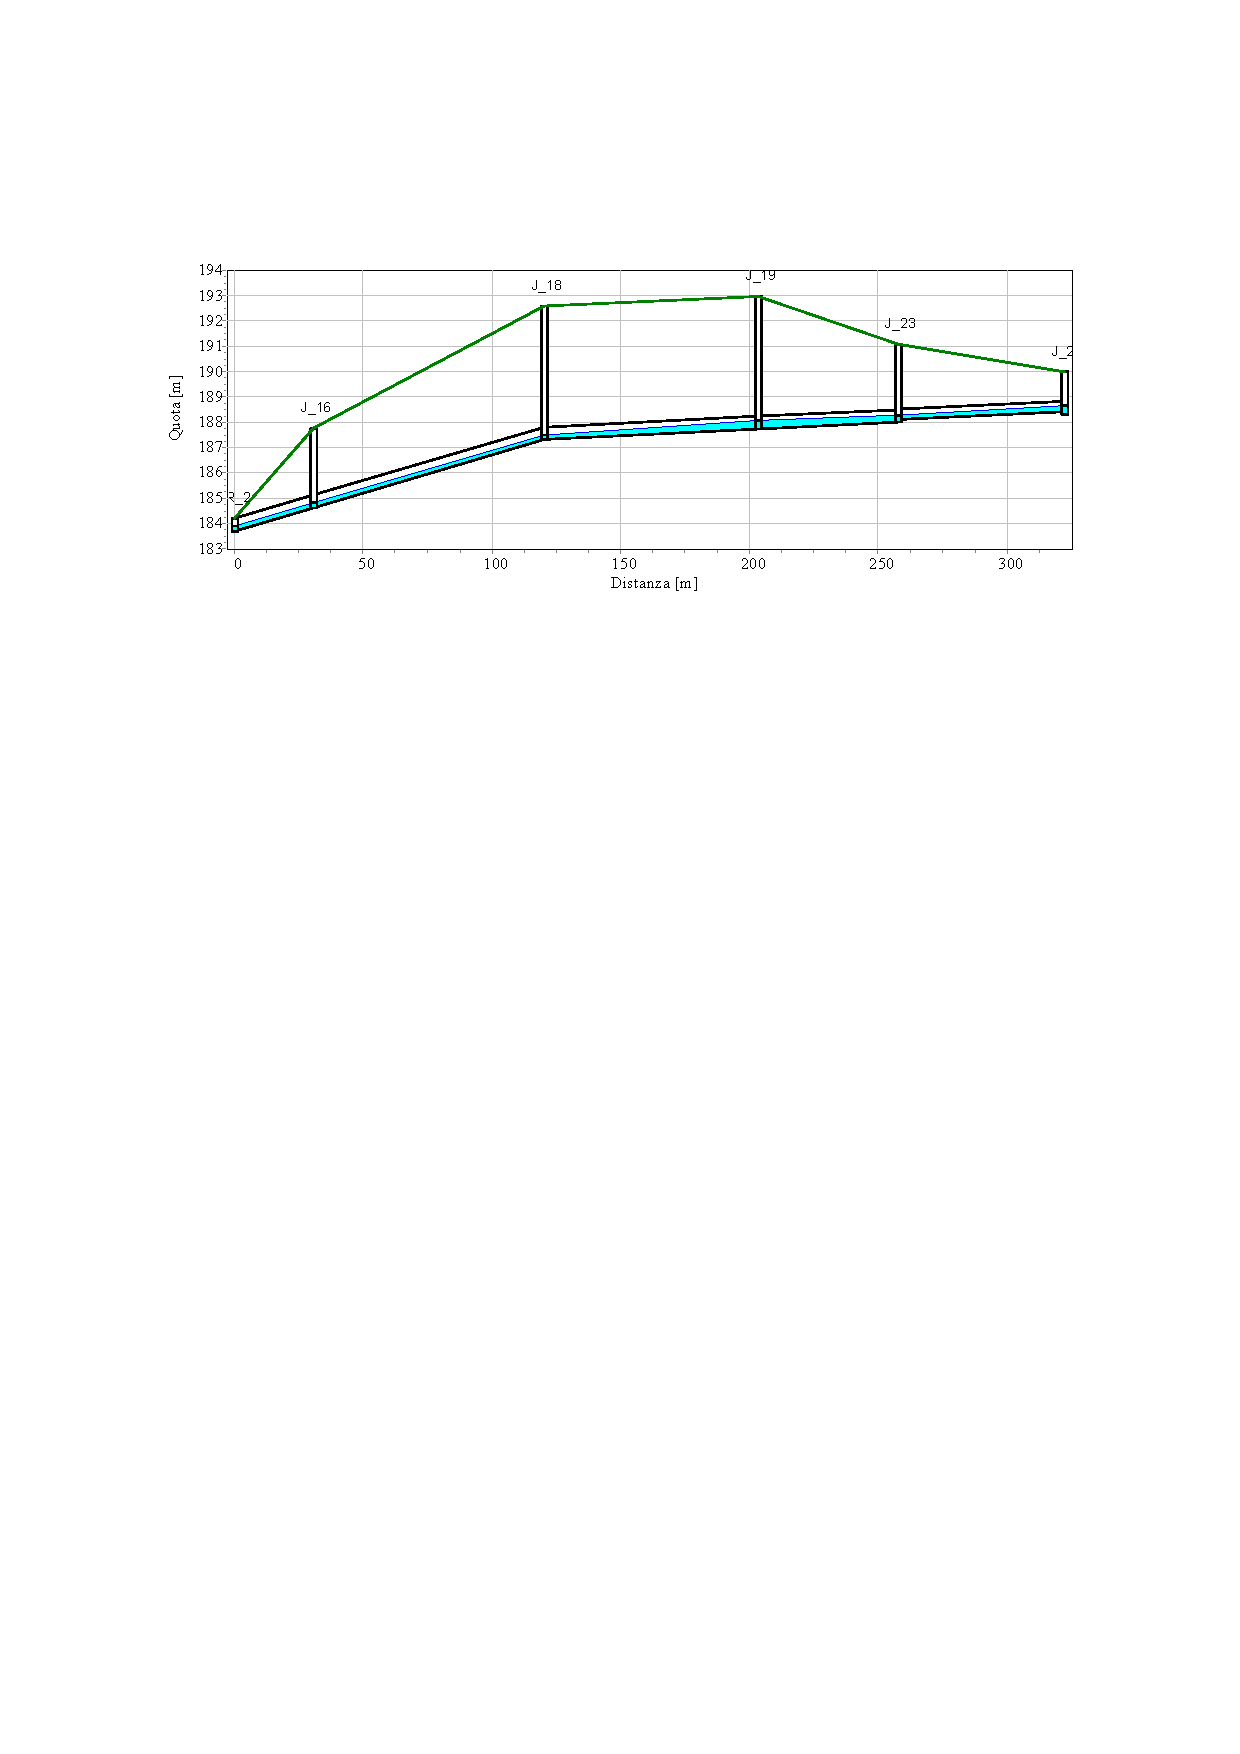
\includegraphics[width=\textwidth]{IMG/ProgettoCondotte_profiloB.pdf}} \\
    \subfloat[][\emph{Ramo di condotte tra il recapito finale 3 ed il tombino $J32$}]{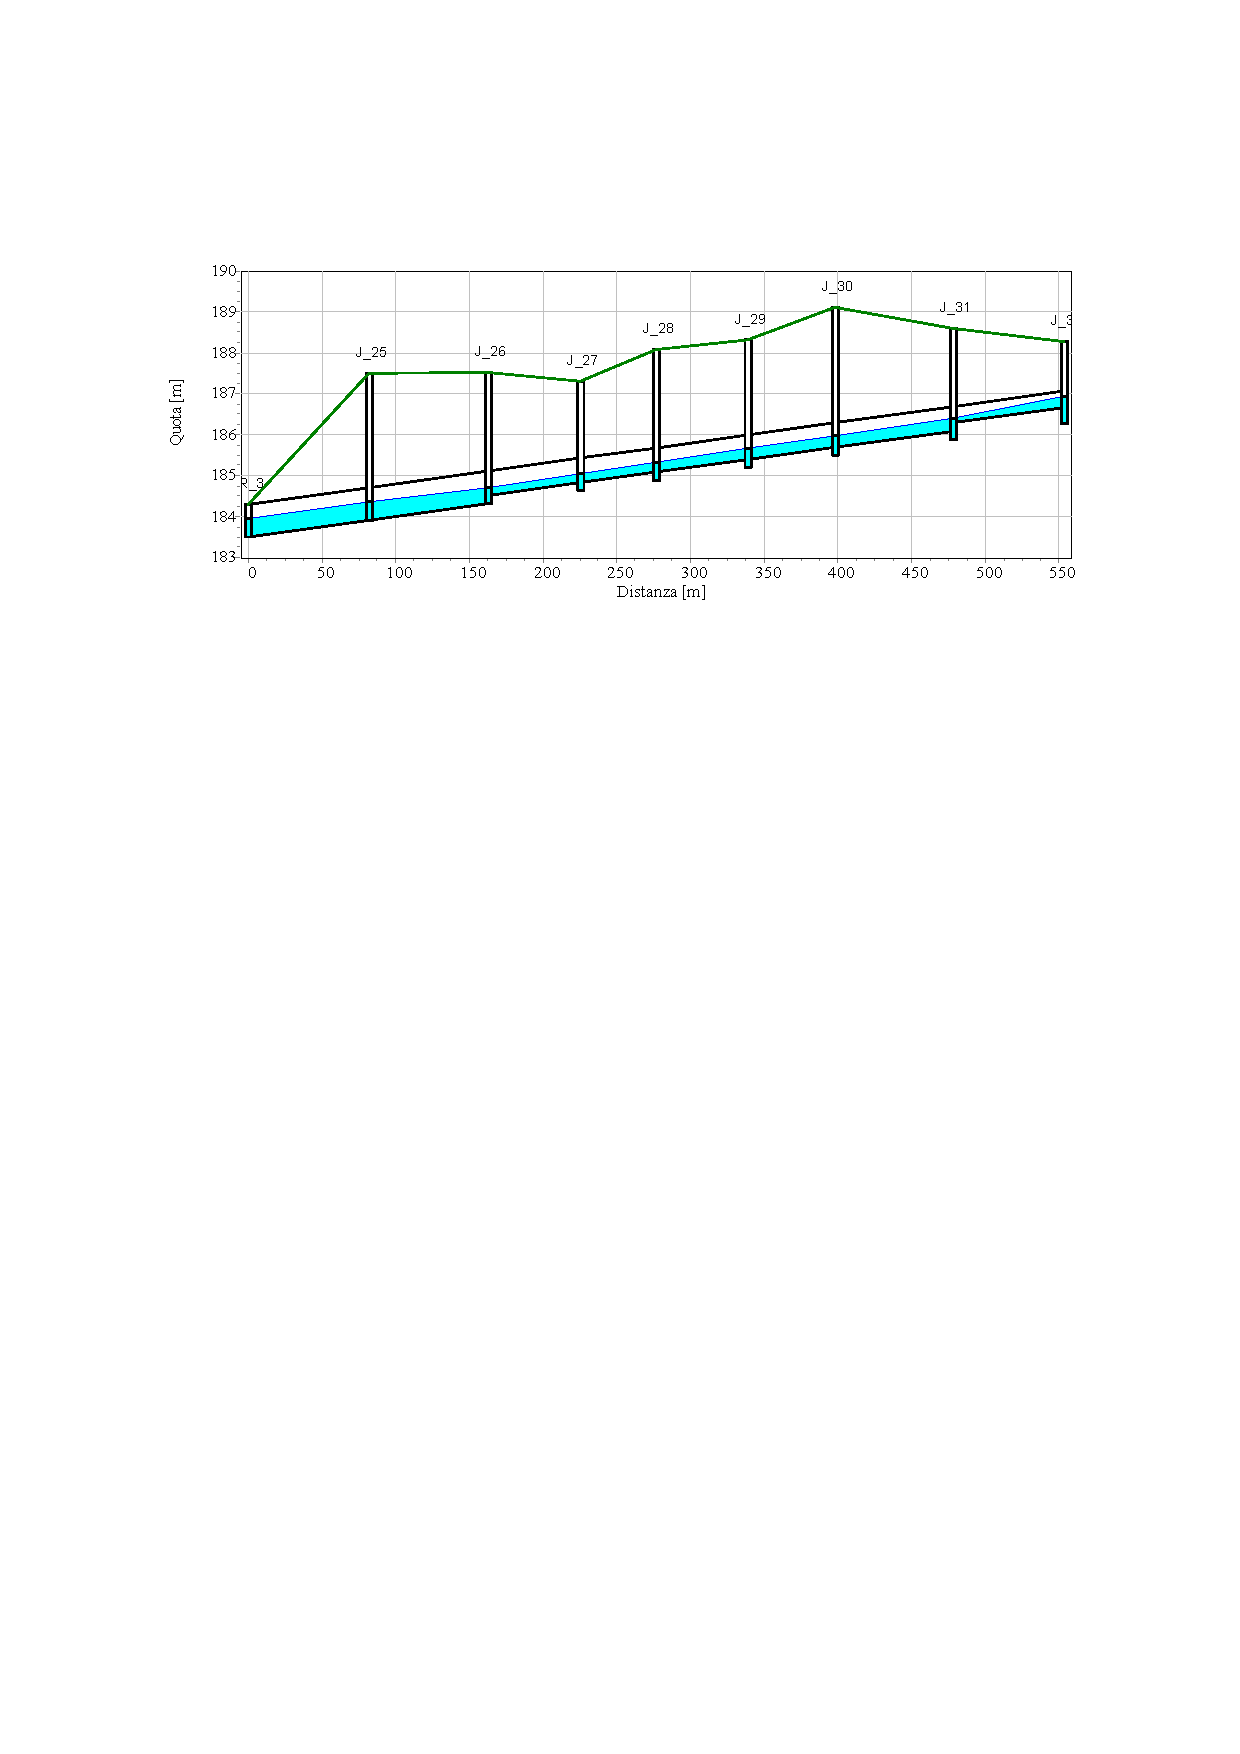
\includegraphics[width=\textwidth]{IMG/ProgettoCondotte_profiloC.pdf}}
\caption{Andamento del pelo libero dell'acqua all'interno delle condotte nell'instante di massimo picco -- Progetto base con solo condotte}
\label{fig:ProfiliProgettoCondotte}
\end{figure}




\end{document}